% Compile with: latexmk -pdfxe -outdir=build
\documentclass[12pt,oneside]{LuThesis}
\usepackage[dvipsnames]{xcolor}
\definecolor{bostonuniversityred}{rgb}{0.8, 0.0, 0.0}
\definecolor{awesome}{rgb}{1.0, 0.13, 0.32}
\definecolor{cadmiumgreen}{rgb}{0.0, 0.42, 0.24}

\usepackage{booktabs}
\usepackage{pythonhighlight}

\title{Daudzvalodīgu jēdzientelpu pielietojums nodomu noteikšanā}
\author{Viktorija Leimane}

%%% LuThesis deklerācijas
\def\studaplnum{vl16047}
\def\darbvad{Dr.sc.comp. Kaspars Balodis}
\def\dokfak{\textbf{Datorikas fakultātē}}
\def\recenzents{Recenzents}
\def\doktitle{\textbf{Daudzvalodīgu jēdzientelpu pielietojums nodomu noteikšanā}}
\def\dokdate{} % Darba vadītāja parakstīšanas datums
\def\dokdateiesn{} % Darba iesniegšanas datums

%%% Valodas un fonti
\setdefaultlanguage{latvian}
\setotherlanguage{english}
\setmainfont[BoldFont=FreeSerifBold.ttf,ItalicFont=FreeSerifItalic.ttf,BoldItalicFont=FreeSerifBoldItalic.ttf]{FreeSerif.ttf}

\usepackage{graphicx}

%%% Misc
% \usepackage{hyperref}
\usepackage[hidelinks]{hyperref}
\addbibresource{thesis.bib} % biblatex bibliotēkas fails: thesis.bib
\usepackage[section]{placeins}
\usepackage[toc,page]{appendix}

%%% Dokumenta struktūra
\begin{document}

\maketitle

% * Anotācija
\chapter*{Anotācija}
\setcounter{page}{1}
\begin{abstract}
Daudzvalodīga lietotāja nodomu noteikšana ir nozīmīga virtuālo asistentu darbībā, un klientu apkalpošanas automatizācija kļūst arvien aktuālāka. Ievades teksta virknes tiek attēlotas daudzdimensionālā vektoru telpā jeb jēdzientelpā, kuru izmanto nodomu klasifikācijas modeļi, lai piegādātu lietotājiem tiem nepieciešamo informāciju. Darbā tiks apmācīti dažādi mašīnmācīšanās modeļi un salīdzinātas dažādas pieejas, piemēram, ievades teksta attēlojums uz daudzvalodīgu tekstu korpusu apmācītas jēdzientelpas vai ievades teksta mašīntulkošana uz angļu valodu pirms jēdzientelpas izveides.

\keywords{daudzvalodīgas jēdzientelpas, nodomu noteikšana}
\end{abstract}

\chapter*{Abstract}
\begin{english}
\begin{abstract}
Multilingual intention detection is important for virtual assistants, and customer-service automation is becoming more cost-effective and relevant. One way of detecting intent is mapping input text strings to multidimensional vector space, which is used by intent classification models to supply users with the information they need. This thesis focuses on training a variety of machine learning models and comparing different approaches, such as mapping input text to multingual word embeddings and machine translating input text to English and using English corpus-based word embeddings for intent detection.

\keywords{multilingual word embeddings, intent detection}


\end{abstract}
\end{english}

%* Saturs
\tableofcontents


\chapter*{Apzīmējumu saraksts}
\addcontentsline{toc}{chapter}{Apzīmējumu saraksts}
NLP (natural language processing) - dabisko valodu apstrāde\\
Jēdzientelpa – (word embeddings) vārdu vai frāžu attēlojums daudzdimensionālā vektoru telpā\\
Word2Vec – (word to vector) jēdzientelpas implementācija, kurā individuālus vārdus aizstāj
daudzimensionāli vektori\\
BERT\\
PCA (principal component analysis) - galveno komponentu analīze


\chapter*{Ievads}
\addcontentsline{toc}{chapter}{Ievads}
Arvien lielāku daļu tirgus pārņem pakalpojumu industrija (\% ES), un pakalpojumi arvien biežāk tiek piedāvāti globāli/starptautiski. Tam ir nepieciešams lietotāju dzimtās valodas atbalsts gan valstu valodu regulējumu, gan tirgus nišas ieņemšanas/tirgus konkurences dēļ (\% ES iedzīvotāju svarīgi saņemt pakalpojumu savā dzimtajā valodā). 

Uzņēmumiem tas galvenokārt ir izdevīgi, jo ļauj samazināt personālizdevumus (\% pakalpojumu nozares uzņēmuma izdevumu). Tas savukārt samazina barjeru dalībai/iekļūšanai starptautiskā tirgū, kas nozīmē lielāku konkurenci un piedāvāto pakalpojumu daudzveidību. Lietotājiem, kuru dzimto valodu pārvalda mazs cilvēku skaits kā tas ir, piemēram, latviešu valodā, ir pieejami pakalpojumi, kuru tulkojumus būtu ekonomiski nerentabli nodrošināt ar algotu profesionālu personālu.

Darbā apskatītā metode nodrošina automatizāciju divos veidos: 
virtuālais asistents aizvieto klientu apkalpošanas speciālistu
daudzvalodīgs modelis aizvieto profesionālu tulkotāju.

Darbs ir sadalīts teorētiskajā un praktiskajā daļā. Teoretiskajā daļā ir īsi
aprakstīti mūsdienu modeļi un pieejas. Praktiskajā daļā ir veikti eksperimenti ar mērķi pielietot daudzvalodīgus modeļus un salīdzināt tos ar esošiem risinājumiem. 


\chapter{Literatūras apskats}
% \section{Definīcijas}
\noindent \textbf{Saules plankums} - magnētiskās plūsmas koncentrācija bipolāros klāsteros vai grupās, kas novērojama kā tumšs plankums uz Saules fotosfēras.\\
\textbf{Saules plankumu cikls} - aptuveni 11 gadus ilga kvaziperiodiska variācija saules plankuma skaitlī. Magnētiskā lauka polaritātes modelis mainās ar katru ciklu.\\
\textbf{Saules plankuma skaitlis} - Dienas saules plankuma aktivitātes indekss (R), definēts kā $R = k(10 \cdot g + s)$, kur
s - individuālo plankumu skaits;
g - saules plankumu grupu skaits;
k - observatorijas faktors.\\
\textbf{SSI} - saules spektrālais starojums vai spektra enerģijas blīvums - saules jaudas izkliede uz virsmas laukuma vienību.\\
% total solar irradiance (TSI) - Solar energy per unit time over a unit area perpendicular to the Sun’s rays at the top of Earth’s atmosphere.
\textbf{TSI} - Saules starojuma absolūtās intensitātes mērījums integrēts visā saules enerģijas diskā un visā saules enerģijas spektrā.\\
% Laboratory for Atmospheric and Space Physics, University of Colorado (2019)
% \\http://lasp.colorado.edu/home/sorce/reference/glossary/
\textbf{Izstarojums} - starojuma avota jaudas incidents uz virsmas laukuma vienību.\\ %Irradiance
\textbf{Saules diennakts kustība} (diurnal motion) - Debess spīdekļu redzamā pārvietošanās pie debess sfēras (rotācija ap pasaules asi) diennakts laikā.\\ %Diurnal motion
% Tās faktiskais cēļonis ir Zemes rotācija ap asi. Diennakts kurstībā visi debess spīdekļi pārvietojas pa debess paralēlēm.
Beam Radiation - the solar radiation received from the sun without having been scattered by the atmosphere (also known as direct solar radiation)
Diffuse Radiation - the solar radiation received from the sun after its direction has been changed by scattering by the atmosphere

\section{Jēdzientelpa}

Jēdzientelpa ir vārdu vai frāžu attēlojums daudzdimensionālā vektoru telpā. Jēdzientelpas no teksta korpusa iegūst ar neironu tīkliem, kuri uztver kontekstu no tuvākajiem vārdiem tekstā. CBOW (Continuous Bag-of-Words) metodē neironu tīkls mēģina uzminēt esošo (vidējo) vārdu no n iepriekšējiem un n nākošajiem vārdiem. Procesu atkārtojot, vārdiem, kas bieži parādās vienā kontekstā, būs līdzīgi vektori. Pēc distributional hypothesis vārdi, kas atrodas līdzīgos kontekstos, ir ar līdzīgu nozīmi.

Atšķirībā no dabisko valodu apstrādes metodēm, kas katru vārdu uztver kā vienu atsevišķu vienību un tādēļ vienīgā iespējamā darbība ar vārdiem ir pārbaudīt vienādību, katras jēdzientelpas vektora vērtības ietekmē vārdi tiem apkārt (distributed representation) un būtībā jēdzientelpas uztver attiecības starp vārdiem. Rezultātā vārdam atbilstošais vektors satur semantisku un sintaktisku informāciju par vārdu. No tā izriet praktiskā implikācija - ar vektoriem var darīt lineāro algebru - saskaitīt, atņemt utml.

Cilvēkiem uztverama jēdzientelpu analoģija ir krāsas nosaukums un tam atbilstošais vektors RGB krāsu modelī ar R, G un B koordinātēm no 0 līdz 255, piemēram, red = (255, 0, 0). Ar krāsu jēdzientelpām ir iespējams veikt saskaitīšanu un atņemšanu, kam ir fizikāla nozīme.

Atrast tuvākās krāsas sarkanam.
\begin{python}
closest(colors, colors['red'])
# red (229, 0, 0)
# fire engine red (254, 0, 2)
# bright red (255, 0, 13)
# tomato red (236, 45, 1)
# cherry red (247, 2, 42)
\end{python}

Operācijas ar vektoriem darbojas gan krāsu nosaukumiem semantiski, gan skaitliskiem vektoriem krāsu telpā. Piemēram, tuvākais vektors violeta un sarkana starpībai ir zils, kas atbilst cilvēku intuīcijai par RGB krāsām.
$$purple - red = blue$$
$$(126, 30, 156) - (229, 0, 0) = (-103, 30, 156)$$
\begin{python}
closest(colors, subtractv(colors['purple'], colors['red']))
# cobalt blue (3, 10, 167)
# royal blue (5, 4, 170)
# darkish blue (1, 65, 130)
# true blue (1, 15, 204)
# royal (12, 23, 147)
\end{python}

Tā saskaitot zaļu un zilu rodas kaut kas pa vidu - tirkīzs.
$$blue + green = turquoise$$
$$(3, 67, 223) + (21, 176, 26) = (24, 243, 249)$$
\begin{python}
closest(colors, addv(colors['blue'], colors['green']))
# bright turquoise (15, 254, 249)
# bright light blue (38, 247, 253)
# bright aqua (11, 249, 234)
# cyan (0, 255, 255)
# neon blue (4, 217, 255)
\end{python}

No vektoru operācijām var nolasīt secinājumus par semantiskajām attiecībām starp vārdiem, piemēram, rozā sarkanam ir tas pats, kas gaiši zils zilam.
$$pink - red + blue = light blue$$
$$(255, 129, 192) - (229, 0, 0) + (3, 67, 223) = (29, 196, 415)$$
\begin{python}
closest(colors, addv(subtractv(colors['pink'], colors['red']), colors['blue']))
# neon blue (4, 217, 255)
# bright sky blue (2, 204, 254)
# bright light blue (38, 247, 253)
# cyan (0, 255, 255)
# bright cyan (65, 253, 254)
\end{python}

%\begin{python}

%\end{python}

Izrādās tādas pašas sakarības kādas ir krāsu nosaukumiem un to attēlojumiem krāsu telpā ir spēkā jebkuram vārdam (ref 1.1. tabula). Vārdi, kuri bieži atrodas līdzīgos kontekstos, ir tuvāki nozīmē. Jēdzientelpas ietver gan sintaktiskas, gan semantiskas attiecības starp vārdiem. Jāuzsver, ka tādas semantiskas attiecības kā valsts-galvaspilsēta nav eksplicīti uzdotas, jēdzientelpu modelis tās ir novērojis tikai balstoties uz vārdu atrašanās vietām teksta korpusā.


Spēja noteikt sintaktisku un semantisku vārdu attiecības ir īpaši būtiska virtuālo asistentu jomā, jo, pirmkārt, semantiski līdzīgiem nodomiem ir līdzīgi vektori, tātad tie vienādi klasificēsies, otrkārt, informācija par sintakses attiecībām noder, jo lietotāji ievada jautājumus brīvā formā un tas ir it īpaši svarīgi fleksīvām valodām kā latviešu.



\begin{table}[htbp]
	\centering
	\caption{Semantisko attiecību piemēri}
	\begin{tabular}{ll}\toprule
		attiecība & piemērs  \\\midrule
		valsts-galvaspilsēta   & Parīze - Francija + Itālija = Roma \\
		valsts-valūta   & dolāri - ASV + Latvija = eiro \\
		vīrietis-sieviete   & karalis - vīrietis + sieviete = karaliene \\\bottomrule
	\end{tabular}%
	\label{tab:semantic-relationship-examples}%
\end{table}

\begin{table}[htbp]
	\centering
	\caption{Sintaktisko attiecību piemēri}
	\begin{tabular}{ll}\toprule
		attiecība & piemērs  \\\midrule
		daudzskaitlis   & pele - peles \\
		pagātne   & staigā - staigāja \\
		salīdzināmā pakāpe   & labs - labāks \\\bottomrule
	\end{tabular}%
	\label{tab:semantic-relationship-examples}%
\end{table}


\begin{figure}[h]
	\centering
	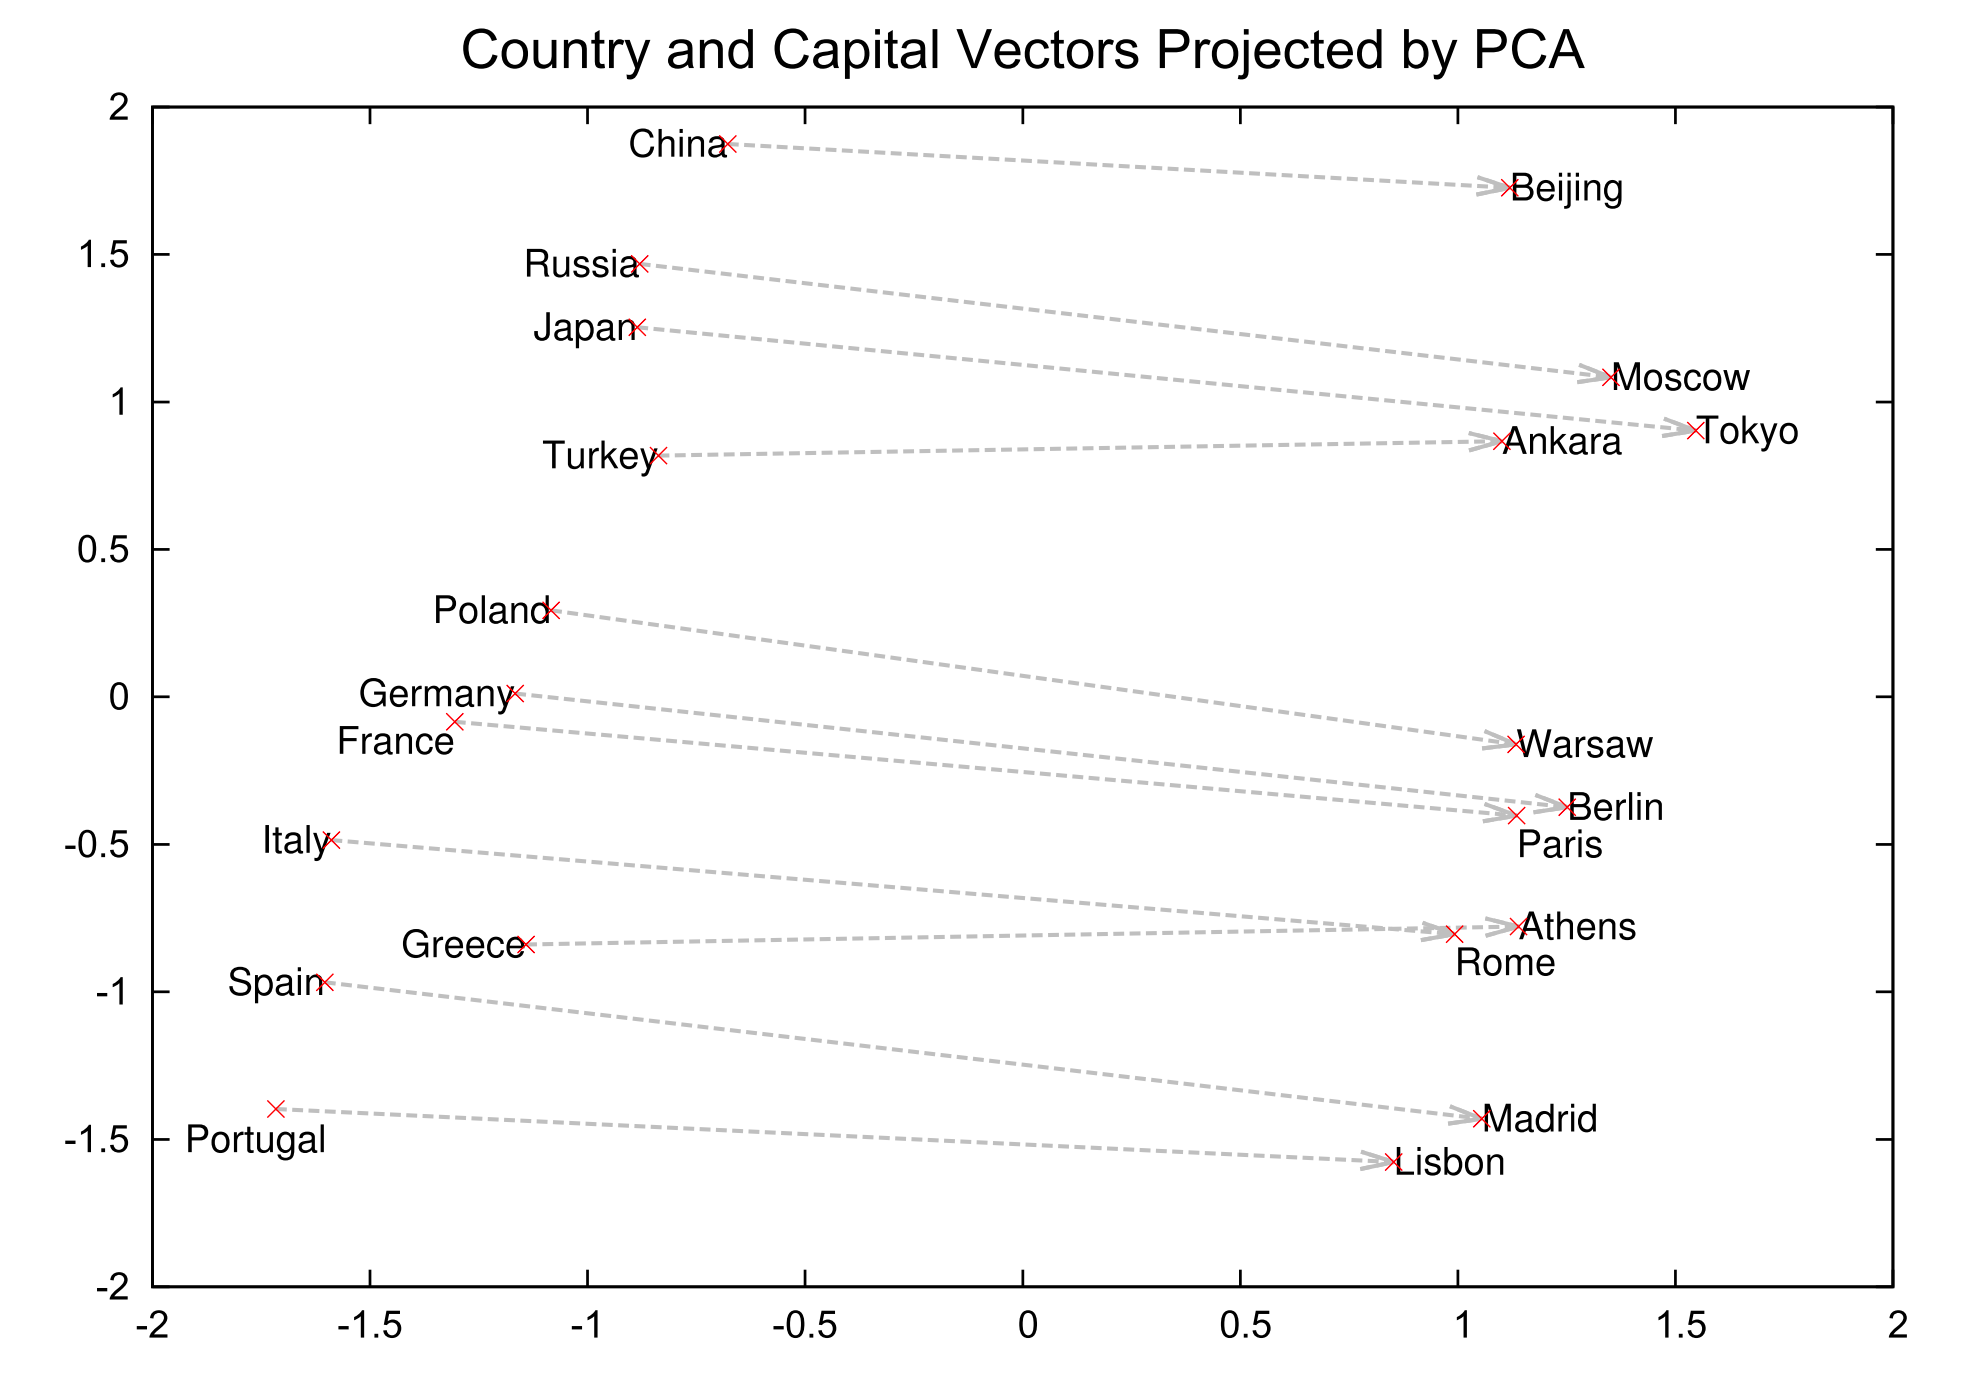
\includegraphics[width=\textwidth]{figures/word2vec-country-capital.png}
	\caption{Divdimensionāla PCA projekcija uzrāda attiecības starp valstu un galvaspilsētu jēdzientelpām}
\end{figure}

%distributed reprezentations
%http://www.cs.toronto.edu/~rgrosse/courses/csc321_2018/readings/L07%20Distributed%20Representations.pdf


% \chapter{Rezultāti}
% 
Šajā nodaļā ir izklāstīti pētījuma rezultāti, kuru mērķis ir salīdzināt dažādu lietotāju nodomu noteikšanas metožu precizitāti angļu, latviešu, krievu, igauņu un lietuviešu valodās, izmantojot mBERT un XLM-RoBERTa jēdzientelpas un dažādu valodu datus. Nodaļā rezultāti tiek analizēti pēc precizitātes un tiek apskatīti modeļu apmācības grafiki. Tāpat nodaļā ir apskatīta iegūto rezultātu ietekme uz virtuālo asistentu sistēmu izstrādi un uzlabošanu.

\ref{tab:legend} tabula sniedz pārskatu par atšķirībām starp dažādām lietotāju nodomu noteikšanai izmantotajām metodēm, pamatojoties uz apmācībā izmantoto valodu un to, vai korpuss ir bijis mašīntulkots uz angļu valodu. Tabulā ir īsi definēti 1a, 1b, 2a, 2b, 3a, 3b metožu apzīmējumi, ļaujot interpretēt turpmākās tabulas ar rezultātiem.


% preferably leave this
\begin{table}[htbp]
  \centering
  \caption{Apkopojums galvenajām atšķirībām starp 1a, 1b, 2a, 2b, 3a, 3b metodēm attiecībā uz apmācības valodu un korpusa valodu (oriģinālvaloda vai mašīntulkojums uz angļu valodu). Alternatīvs caption: 1a, 1b, 2a, 2b, 3a, 3b metožu abreviatūru atšifrējums.}
  % \caption{1a, 1b, 2a, 2b, 3a, 3b metožu abreviatūru atšifrējums.}
    \begin{tabular}{lll}\toprule
    Abreviatūra & Apmācības valoda & Korpusa valoda \\\midrule
    1a    & \multicolumn{1}{l}{\multirow{2}[0]{*}{Apmācība vienā valodā}} & mašīntulkoti angļu valodā \\
    1b    &       & oriģinālvalodā \\\midrule
    2a    & \multicolumn{1}{l}{\multirow{2}[0]{*}{Apmācība uz visām valodām}} & mašīntulkoti angļu valodā \\
    2b    &       & oriģinālvalodā \\\midrule
    3a    & \multicolumn{1}{l}{\multirow{2}[0]{*}{Apmācība tikai angļu valodā}} & mašīntulkoti angļu valodā \\
    3b    &       & oriģinālvalodā \\\bottomrule
    \end{tabular}%
  \label{tab:legend}%
\end{table}%


% Table generated by Excel2LaTeX from sheet 'Sheet1'
\begin{table}[htbp]
  \centering
  \caption{Apkopojums galvenajām atšķirībām starp 1a, 1b, 2a, 2b, 3a, 3b metodēm attiecībā uz apmācības valodu un ievaddatu valodu.}
    \begin{tabular}{ll}\toprule
    Abreviatūra & Atšifrējums \\\midrule
    1 & Apmācība un testēšana vienā valodā \\
    2 & Apmācība uz visām valodām, testēšana vienā valodā \\
    3 & Apmācība angļu valodā, testēšana valodās, kas nav angļu \\\midrule
    a & mašīntulkoti angļu valodā \\
    b & oriģinālvalodā \\\bottomrule
    \end{tabular}%
  \label{tab:legend}%
\end{table}%



\section{Chatbot datu kopa}

Tabulā \ref{tab:chatbot-labels} ir sniegta informācija par unikālo nodomu skaitu  \textit{Chatbot} treniņkopā un testa kopā, kā arī to summa.

\begin{table}[htbp]
  \centering
  \caption{Unikālo nodomu skaits "chatbot" treniņkopā un testa kopā.}
    \begin{tabular}{lrrr} \toprule
    Nodoms & Treniņkopā & Testa kopā & $\Sigma$ \\\midrule
    FindConnection & 57    & 71 & 128 \\
    DepartureTime & 43    & 35 & 78 \\
    $\Sigma$ & 100    & 106 & 206 \\\bottomrule
    \end{tabular}%
  \label{tab:chatbot-labels}%
\end{table}%


Nodomu noteikšanas precizitāte \textit{Chatbot} datu kopā ir apkopota pēc izmantotā jēdzientelpu modeļa: mBERT (\ref{tab:chatbot-bert} tabula) un XLM-RoBERTa (\ref{tab:chatbot-xlm} tabula). Salīdzinot šīs jēdzientelpas, redzams, ka angļu valodā uz XLM-RoBERTa jēdzientelpām precizitāte ir augstāka, bet lietuviešu valodā -- zemāka nekā mBERT jēdzientelpām. Kopumā mBERT un XLM-RoBERTa modeļi uzrāda līdzīgus rezultātus.
% Kopumā rezultāti liecina, ka XLM-RoBERTa jēdzientelpas ir piemērotākas nodomu noteikšanai Chatbot datu kopā.

% Kopumā rezultāti liecina, ka XLM-RoBERT pārspēja mBERT lielākajā daļā scenāriju un valodu.
% Stratēģijā, kas apmāca tikai uz angļu valodas datiem un testē citā valodā:

Igauņu valodā ir vislielākais kritums stratēģijā, kas apmāca tikai uz angļu valodas datiem un testē igauņu valodā, tas atbilst paredzētajam, jo igauņu valoda ir vismazāk pārstāvēta korpusos, uz kuriem apmācīti mBERT un XLM-RoBERTa modeļi. Lai gan intuitīvi varētu šķist, ka modelis, kas apmācīts tikai angļu valodā, slikti spēs klasificēt nodomus citā valodā, rezultāti pierāda pretējo -- 3b kolonnā redzami salīdzinoši labi rezultāti uz testa kopām krievu un latviešu valodās (85.85--93.40\%). Tas tādēļ, ka daudzvalodu jēdzientelpas angļu datu kopās ir līdzīgas tādu pašu teikumu jēdzientelpām citās valodās.


% maz-resursu valodas iegūst no tulkošanas uz angļu valodu

% Vidēji latviešu valodas mašīntulkojums uz angļu valodu ir ar lielāku precizitāti nekā oriģinālvalodā (1ab--2ab) abās jēdzientelpās, taču krievu valodas korpusa tulkojums uz angļu valodu precizitāti zaudēja. 

Vidēji, izmantojot latviešu valodas mašīntulkojumus uz angļu valodu, var sasniegt lielāku precizitāti nekā oriģinālvalodā (1ab--2ab) abās jēdzientelpās, taču krievu valodas korpusa tulkojums uz angļu valodu precizitāti samazināja. Gadījumā, kad modelis apmācīts tikai uz angļu valodas korpusa, precizitāte būtiski uzlabojos testa kopu mašīntulkojot uz angļu valodu, igauņu un lietuviešu valodās precizitātei vidēji pieaugot par 30\% un 12\% attiecīgi, izņemot krievu valodu, kur precizitāte mazliet samazinās -- par 3.8\% mBERT un 1\% XLM-RoBERTa jēdzientelpām. Šo izņēmumu krievu valodā varētu izskaidrot tās salīdzinoši labā pārstāvētība korpusos, uz kuriem apmācīti mBERT un XLM-RoBERTa modeļi, salīdzinot ar latviešu, igauņu un lietuviešu valodām (\ref{fig:dataset-size} attēls).


% Maz-resursu valodās (latviešu, lietuviešu, igauņu) mašīntulkošana angļu valodā galvenokārt uzlaboja precizitāti (1ab).

Maz-resursu valodās (latviešu, lietuviešu, igauņu) tipiski precizitāte ieguva no apmācības uz datiem, kas mašīntulkoti angļu valodā (1ab). Visās valodās visstabilākā veiktspēja ir metodei, kas apmāca modeli uz visām valodām apvienotām vienā korpusā (2ab), kas nebūtiski atšķiras no tā, vai dati pirms tam ir mašīntulkoti uz angļu valodu.

% Table generated by Excel2LaTeX from sheet 'chatbot_bert-base-multilingual-'
% \begin{table}[htbp]
%   \centering
%   \caption{Nodomu noteikšanas precizitāte uz \textit{Chatbot} datukopas ar mBERT modeli, \%}
%   % \caption{mBERT rezultāti}
%     \begin{tabular}{lrrrrrr} \toprule
%     languages & 1a & 1b & 2a & 2b & 3a & 3b \\\midrule
%     en    &   --  & 91.51 &  --   & 90.57 &  --   & 95.28 \\
%     lv    & 90.57 & 88.68 & 94.34 & 93.40 & 92.45 & 85.85 \\
%     ru    & 89.62 & 92.45 & 93.40 & 91.51 & 89.62 & 93.40 \\
%     et    & 89.62 & 87.74 & 86.79 & 88.68 & 90.57 & 58.49 \\
%     lt    & 95.28 & 94.34 & 94.34 & 94.34 & 91.51 & 79.25 \\\bottomrule
%     \end{tabular}%
%   \label{tab:chatbot-bert}%
% \end{table}%

% Table generated by Excel2LaTeX from sheet 'chatbot_bert-base-multilingual-'
\begin{table}[htbp]
  \centering
  \caption{Nodomu noteikšanas precizitāte uz \textit{Chatbot} datukopas ar mBERT modeli, \%}
  % \caption{mBERT rezultāti}
    \begin{tabular}{lrrrrrr} \toprule
    languages & 1a & 1b & 2a & 2b & 3a & 3b \\\midrule
    en    &  --   & \cellcolor[rgb]{ .988,  .988,  1}91.51 &    -- & \cellcolor[rgb]{ .984,  .969,  .98}90.57 &  --   & \cellcolor[rgb]{ .353,  .541,  .776}95.28 \\
    lv    & \cellcolor[rgb]{ .984,  .969,  .98}90.57 & \cellcolor[rgb]{ .984,  .937,  .949}88.68 & \cellcolor[rgb]{ .514,  .655,  .835}94.34 & \cellcolor[rgb]{ .671,  .765,  .89}93.40 & \cellcolor[rgb]{ .831,  .878,  .945}92.45 & \cellcolor[rgb]{ .984,  .886,  .898}85.85 \\
    ru    & \cellcolor[rgb]{ .984,  .953,  .965}89.62 & \cellcolor[rgb]{ .831,  .878,  .945}92.45 & \cellcolor[rgb]{ .671,  .765,  .89}93.40 & \cellcolor[rgb]{ .988,  .988,  1}91.51 & \cellcolor[rgb]{ .984,  .953,  .965}89.62 & \cellcolor[rgb]{ .671,  .765,  .89}93.40 \\
    et    & \cellcolor[rgb]{ .984,  .953,  .965}89.62 & \cellcolor[rgb]{ .984,  .922,  .933}87.74 & \cellcolor[rgb]{ .984,  .906,  .914}86.79 & \cellcolor[rgb]{ .984,  .937,  .949}88.68 & \cellcolor[rgb]{ .984,  .969,  .98}90.57 & \cellcolor[rgb]{ .973,  .412,  .42}58.49 \\
    lt    & \cellcolor[rgb]{ .353,  .541,  .776}95.28 & \cellcolor[rgb]{ .514,  .655,  .835}94.34 & \cellcolor[rgb]{ .514,  .655,  .835}94.34 & \cellcolor[rgb]{ .514,  .655,  .835}94.34 & \cellcolor[rgb]{ .988,  .988,  1}91.51 & \cellcolor[rgb]{ .98,  .773,  .784}79.25 \\\bottomrule
    avg   & 91.27 & 90.94 & 92.22 & 91.70 & 91.04 & 82.45 \\
    % avg en-ru & 89.62 & 91.98 & 93.40 & 91.04 & 89.62 & 94.34 \\
    avg lv-lt-et & 91.82 & 90.25 & 91.82 & 92.14 & 91.51 & 74.53 \\
    \end{tabular}%
  \label{tab:chatbot-bert}%
\end{table}%



% Table generated by Excel2LaTeX from sheet 'chatbot_xlm-roberta-base_result'
% \begin{table}[htbp]
%   \centering
%   \caption{Nodomu noteikšanas precizitāte uz \textit{Chatbot} datukopas ar XLM-RoBERTa modeli, \%}
%   % \caption{Add caption}
%     \begin{tabular}{lrrrrrr} \toprule
%     languages & 1a & 1b & 2a & 2b & 3a & 3b \\\midrule
%     en    &   --  & 95.28 &   --  & 95.28 &  --   & 96.23 \\
%     lv    & 91.51 & 88.68 & 93.40 & 93.40 & 94.34 & 85.85 \\
%     ru    & 92.45 & 94.34 & 88.68 & 94.34 & 91.51 & 90.57 \\
%     et    & 88.68 & 91.51 & 88.68 & 89.62 & 91.51 & 63.21 \\
%     lt    & 92.45 & 91.51 & 91.51 & 93.40 & 90.57 & 77.36 \\\bottomrule
%     \end{tabular}%
%   \label{tab:chatbot-xlm}%
% \end{table}%


% Table generated by Excel2LaTeX from sheet 'chatbot_xlm-roberta-base_result'
\begin{table}[htbp]
  \centering
  \caption{Nodomu noteikšanas precizitāte uz \textit{Chatbot} datukopas ar XLM-RoBERTa modeli, \%}
    \begin{tabular}{lrrrrrr} \toprule
    languages & 1a & 1b & 2a & 2b & 3a & 3b \\\midrule
    en    &   --  & \cellcolor[rgb]{ .482,  .631,  .824}95.28 &  --   & \cellcolor[rgb]{ .482,  .631,  .824}95.28 &  --   & \cellcolor[rgb]{ .353,  .541,  .776}96.23 \\
    lv    & \cellcolor[rgb]{ .988,  .988,  1}91.51 & \cellcolor[rgb]{ .984,  .929,  .941}88.68 & \cellcolor[rgb]{ .737,  .812,  .914}93.40 & \cellcolor[rgb]{ .737,  .812,  .914}93.40 & \cellcolor[rgb]{ .608,  .722,  .867}94.34 & \cellcolor[rgb]{ .984,  .871,  .882}85.85 \\
    ru    & \cellcolor[rgb]{ .863,  .902,  .957}92.45 & \cellcolor[rgb]{ .608,  .722,  .867}94.34 & \cellcolor[rgb]{ .984,  .929,  .941}88.68 & \cellcolor[rgb]{ .608,  .722,  .867}94.34 & \cellcolor[rgb]{ .988,  .988,  1}91.51 & \cellcolor[rgb]{ .984,  .969,  .98}90.57 \\
    et    & \cellcolor[rgb]{ .984,  .929,  .941}88.68 & \cellcolor[rgb]{ .988,  .988,  1}91.51 & \cellcolor[rgb]{ .984,  .929,  .941}88.68 & \cellcolor[rgb]{ .984,  .949,  .961}89.62 & \cellcolor[rgb]{ .988,  .988,  1}91.51 & \cellcolor[rgb]{ .973,  .412,  .42}63.21 \\
    lt    & \cellcolor[rgb]{ .863,  .902,  .957}92.45 & \cellcolor[rgb]{ .988,  .988,  1}91.51 & \cellcolor[rgb]{ .988,  .988,  1}91.51 & \cellcolor[rgb]{ .737,  .812,  .914}93.40 & \cellcolor[rgb]{ .984,  .969,  .98}90.57 & \cellcolor[rgb]{ .98,  .698,  .71}77.36 \\\bottomrule
    avg   & 91.27 & 92.26 & 90.57 & 93.21 & 91.98 & 82.64 \\
    % avg en-ru & 92.45 & 94.81 & 88.68 & 94.81 & 91.51 & 93.40 \\
    avg lv-lt-et & 90.88 & 90.57 & 91.19 & 92.14 & 92.14 & 75.47 \\
    \end{tabular}%
  \label{tab:chatbot-xlm}%
\end{table}%



Att.~\ref{fig:chatbot-bert} parāda precizitāti apmācības laikā, lietojot mBERT jēdzientelpu un treniņdatus latviešu valodā. Redzams, ka apmācības laiks (epochs) bija nepietiekams (att.~\ref{fig:chatbot-bert}, pa labi), jo trenēšanās pārtrūka pie treniņkopas precizitātes 90\%, kad vairums citos grafikos tas sasniedza 100\%. Tas vieš cerības, ka palielinot epochs skaitu 1a un 1b scenārijos, izdotos iegūt augstāku precizitāti. Mašīntulkoto datu gadījumā trenēšanās laiks bija pietiekams (att.~\ref{fig:chatbot-bert}, pa labi), un arī precizitāte uz testa kopas ir mazliet augstāka -- 91.51\% salīdzinot ar 88.67\%.

\begin{figure}[h] 
   \centering
   \subcaptionbox{mBERT latviešu treniņdatu kopa}{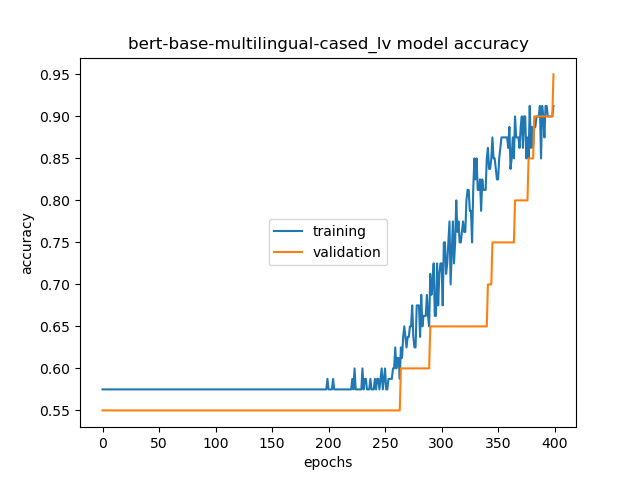
\includegraphics[width=0.49\linewidth,trim={0 0.1cm 0 0},clip]{graphs/bert-base-multilingual-cased_lv-accuracy.png}}
   \subcaptionbox{mBERT mašīntulkoto latviešu treniņdatu kopa}{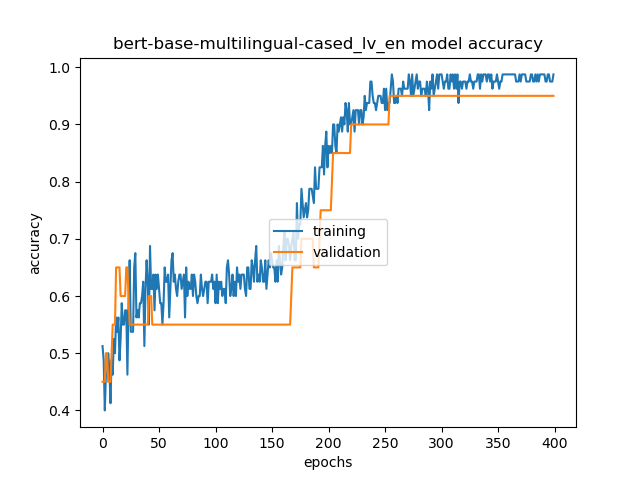
\includegraphics[width=0.49\linewidth,trim={0 0.1cm 0 0},clip]{graphs/bert-base-multilingual-cased_lv_en-accuracy.png}}
   \caption{caption} 
   \label{fig:chatbot-bert}
\end{figure}


\begin{figure}[h] 
   \centering
   \subcaptionbox{mBERT apvienotā treniņdatu kopa}{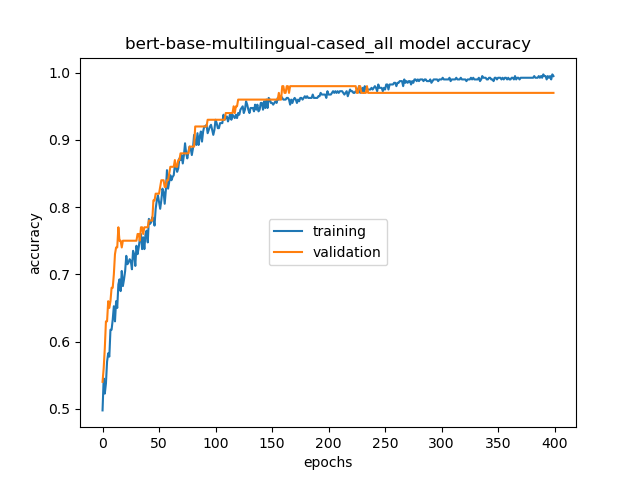
\includegraphics[width=0.49\linewidth,trim={0 0.1cm 0 0},clip]{graphs/bert-base-multilingual-cased_all-accuracy.png}}
   \subcaptionbox{mBERT apvienotā mašīntulkoto treniņdatu kopa}{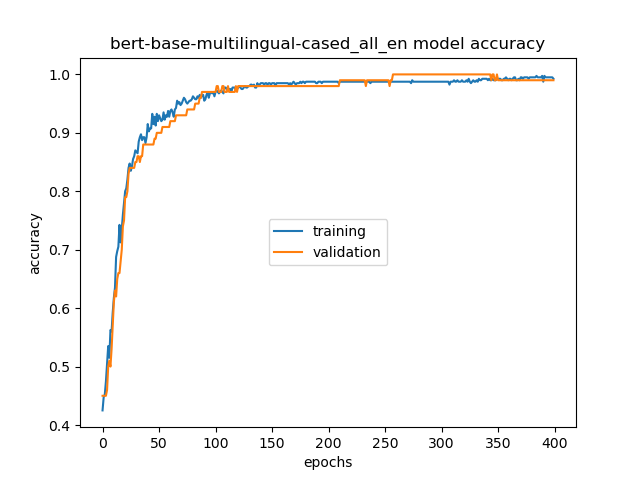
\includegraphics[width=0.49\linewidth,trim={0 0.1cm 0 0},clip]{graphs/bert-base-multilingual-cased_all_en-accuracy.png}}
   \caption{caption} 
   \label{fig:chatbot-bert-all}
\end{figure}


\begin{figure}[h] 
   \centering
   \subcaptionbox{mBERT angļu treniņdatu kopa}{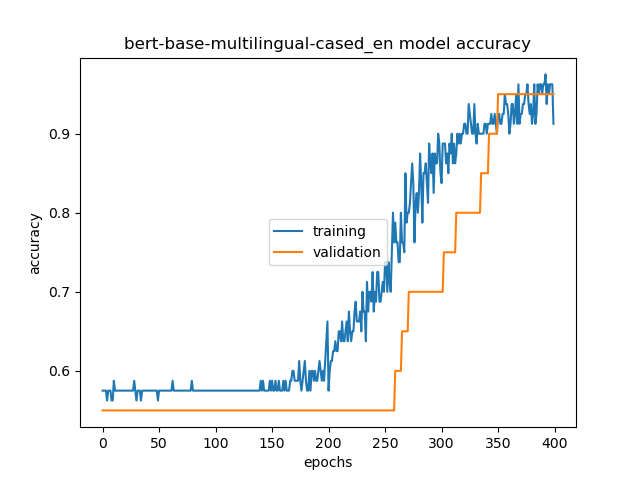
\includegraphics[width=0.49\linewidth,trim={0 0.1cm 0 0},clip]{graphs/bert-base-multilingual-cased_en-accuracy.png}}
   \subcaptionbox{XLM-RoBERTa angļu treniņdatu kopa}{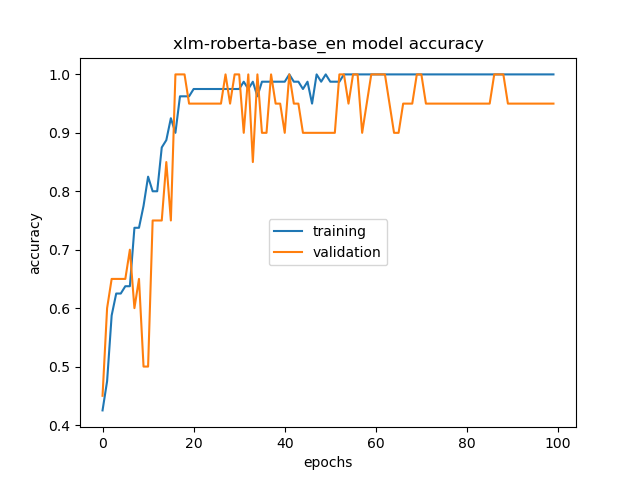
\includegraphics[width=0.49\linewidth,trim={0 0.1cm 0 0},clip]{graphs/xlm-roberta-base_en-accuracy.png}}
   \caption{caption} 
   \label{fig:chabot-bert-xlm-en}
\end{figure}


\begin{figure}[h] 
   \centering
   \subcaptionbox{XLM-RoBERTa latviešu treniņdatu kopa}{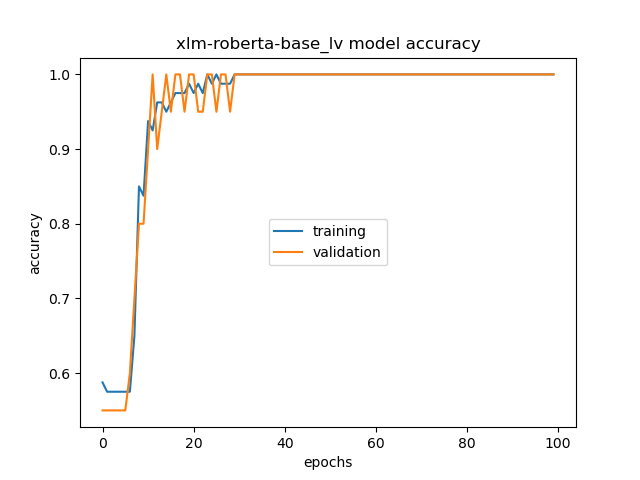
\includegraphics[width=0.49\linewidth,trim={0 0.1cm 0 0},clip]{graphs/xlm-roberta-base_lv-accuracy.png}}
   \subcaptionbox{XLM-RoBERTa mašīntulkoto latviešu treniņdatu kopa}{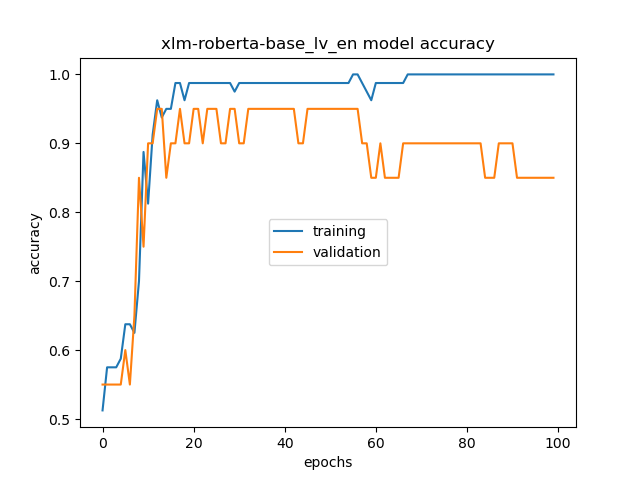
\includegraphics[width=0.49\linewidth,trim={0 0.1cm 0 0},clip]{graphs/xlm-roberta-base_lv_en-accuracy.png}}
   \caption{caption} 
   \label{fig:chatbot-xlm}
\end{figure}


\begin{figure}[h] 
   \centering
   \subcaptionbox{XLM-RoBERTa apvienotā treniņdatu kopa}{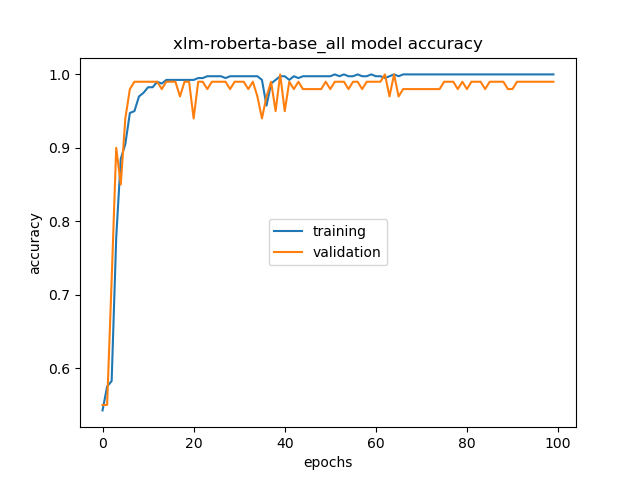
\includegraphics[width=0.49\linewidth,trim={0 0.1cm 0 0},clip]{graphs/xlm-roberta-base_all-accuracy.png}}
   \subcaptionbox{XLM-RoBERTa apvienotā mašīntulkoto treniņdatu kopa}{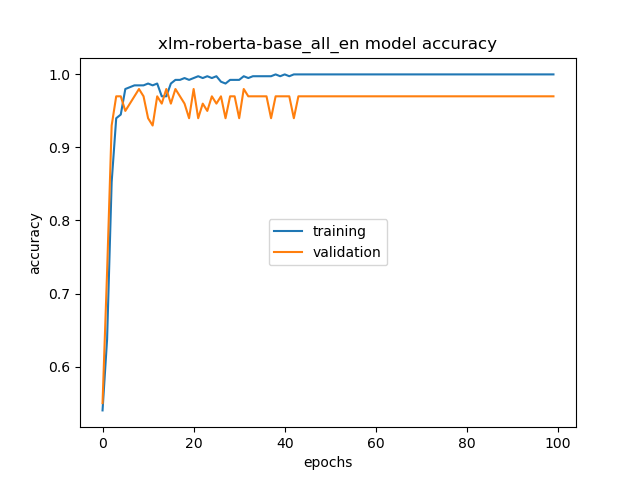
\includegraphics[width=0.49\linewidth,trim={0 0.1cm 0 0},clip]{graphs/xlm-roberta-base_all_en-accuracy.png}}
   \caption{caption} 
   \label{fig:chatbot-xlm-all}
\end{figure}


\section{Askubuntu datu kopa}

\begin{table}[htbp]
  \centering
  \caption{Unikālo nodomu skaits "askubuntu" treniņkopā un testa kopā.}
    \begin{tabular}{lrrr} \toprule
    Nodoms & Treniņkopā & Testa kopā & $\Sigma$ \\\midrule
    Software Recommendation & 17    & 40 & 57 \\
    Make Update & 10    & 37 & 47 \\
    Shutdown Computer & 13    & 14 & 27 \\
    Setup Printer & 10    & 13 & 23\\
    None  & 3     & 5 & 8\\
   $\Sigma$ & 53    & 109 & 162 \\\bottomrule
    \end{tabular}%
  \label{tab:askubuntu-labels}%
\end{table}%



Sliktākā nodomu noteikšanas precizitāte Askubuntu datukopā ir 45.87\%, tas nozīmē, ka modelis modelis pareizi identificēs lietotāja nodomu mazāk nekā puse gadījumos. Lai gan tā ir salīdzinoši zema precizitāte, ir svarīgi atzīmēt, ka datu kopā ir pieci nodomi un, ja nodomi tiktu izvēlēti nejauši, paredzamā precizitāte būtu tikai 20\%. Tāpēc modelis ar 45.87\% precizitātes līmeni joprojām darbojas ievērojami labāk nekā random.

Askubuntu datu kopā nodomu noteikšanas precizitāte ir zemāka nekā Chatbot datu kopā tādeļ, ka ir vairāk nodomu ar mazāk piemēriem katram nodomam.

Datu kopā \textit{Askubuntu} 3b metodei vienmēr bija viszemākā nodomu noteikšanas precizitāte gan mBERT, gan XLM-RoBERTa modeļiem. Turpretim visaugstākā veiktspēja nodomu noteikšanas precizitātē tika sasniegta ar 2b metodi, kam sekoja 3a un 1b metode gan mBERT, gan XLM-RoBERTa modeļiem.



% Table generated by Excel2LaTeX from sheet 'askubuntu_bert-base-multilingua'
\begin{table}[htbp]
  \centering
  \caption{Nodomu noteikšanas precizitāte uz \textit{Askubuntu} datukopas ar mBERT modeli, \%}
    \begin{tabular}{lrrrrrr} \toprule
    languages & 1a & 1b & 2a & 2b & 3a & 3b \\\midrule
    en    &  --   & \cellcolor[rgb]{ .984,  .965,  .976}78.90 &   --  & \cellcolor[rgb]{ .737,  .812,  .914}81.65 &  --   & \cellcolor[rgb]{ .608,  .722,  .867}82.57 \\
    lv    & \cellcolor[rgb]{ .984,  .965,  .976}78.90 & \cellcolor[rgb]{ .737,  .812,  .914}81.65 & \cellcolor[rgb]{ .988,  .988,  1}79.82 & \cellcolor[rgb]{ .353,  .541,  .776}84.40 & \cellcolor[rgb]{ .863,  .902,  .957}80.73 & \cellcolor[rgb]{ .973,  .412,  .42}54.13 \\
    ru    & \cellcolor[rgb]{ .482,  .631,  .824}83.49 & \cellcolor[rgb]{ .737,  .812,  .914}81.65 & \cellcolor[rgb]{ .984,  .882,  .894}75.23 & \cellcolor[rgb]{ .737,  .812,  .914}81.65 & \cellcolor[rgb]{ .988,  .988,  1}79.82 & \cellcolor[rgb]{ .976,  .655,  .667}65.14 \\
    et    & \cellcolor[rgb]{ .984,  .965,  .976}78.90 & \cellcolor[rgb]{ .482,  .631,  .824}83.49 & \cellcolor[rgb]{ .737,  .812,  .914}81.65 & \cellcolor[rgb]{ .984,  .925,  .937}77.06 & \cellcolor[rgb]{ .984,  .965,  .976}78.90 & \cellcolor[rgb]{ .973,  .494,  .502}57.80 \\
    lt    & \cellcolor[rgb]{ .608,  .722,  .867}82.57 & \cellcolor[rgb]{ .984,  .945,  .957}77.98 & \cellcolor[rgb]{ .984,  .965,  .976}78.90 & \cellcolor[rgb]{ .98,  .824,  .831}72.48 & \cellcolor[rgb]{ .863,  .902,  .957}80.73 & \cellcolor[rgb]{ .973,  .533,  .541}59.63 \\\bottomrule
    avg   & 80.96 & 80.73 & 78.90 & 79.45 & 80.05 & 63.85 \\
    % avg en-ru & 83.49 & 80.28 & 75.23 & 81.65 & 79.82 & 73.85 \\
    ang rest & 80.12 & 81.04 & 80.12 & 77.98 & 80.12 & 57.19 \\
    \end{tabular}%
  \label{tab:askubuntu-bert}%
\end{table}%


% uncolored just in case
% Table generated by Excel2LaTeX from sheet 'askubuntu_bert-base-multilingua'
% \begin{table}[htbp]
%   \centering
%     \caption{Nodomu noteikšanas precizitāte uz \textit{Askubuntu} datukopas ar mBERT modeli, \%}
%     \begin{tabular}{lrrrrrr} \toprule
%     languages & 1a & 1b & 2a & 2b & 3a & 3b \\\midrule
%     en    &   --  & 78.90 &   --  & 81.65 &  --   & 82.57 \\
%     lv    & 78.90 & 81.65 & 79.82 & 84.40 & 80.73 & 54.13 \\
%     ru    & 83.49 & 81.65 & 75.23 & 81.65 & 79.82 & 65.14 \\
%     et    & 78.90 & 83.49 & 81.65 & 77.06 & 78.90 & 57.80 \\
%     lt    & 82.57 & 77.98 & 78.90 & 72.48 & 80.73 & 59.63 \\\bottomrule
%     \end{tabular}%
%   \label{tab:askubuntu-bert}%
% \end{table}%


% Table generated by Excel2LaTeX from sheet 'askubuntu_xlm-roberta-base_resu'
\begin{table}[htbp]
  \centering
  \caption{Nodomu noteikšanas precizitāte uz \textit{Askubuntu} datukopas ar XLM-RoBERTa modeli, \%}
    \begin{tabular}{lrrrrrr}\toprule
    languages & 1a & 1b & 2a & 2b & 3a & 3b \\\midrule
    en    &   --  & \cellcolor[rgb]{ .498,  .643,  .827}77.06 &  --   & \cellcolor[rgb]{ .353,  .541,  .776}78.90 &   --  & \cellcolor[rgb]{ .988,  .988,  1}70.64 \\
    lv    & \cellcolor[rgb]{ .984,  .922,  .933}67.89 & \cellcolor[rgb]{ .98,  .816,  .827}63.30 & \cellcolor[rgb]{ .353,  .541,  .776}78.90 & \cellcolor[rgb]{ .353,  .541,  .776}78.90 & \cellcolor[rgb]{ .639,  .741,  .878}75.23 & \cellcolor[rgb]{ .973,  .451,  .459}47.71 \\
    ru    & \cellcolor[rgb]{ .984,  .922,  .933}67.89 & \cellcolor[rgb]{ .78,  .843,  .929}73.39 & \cellcolor[rgb]{ .639,  .741,  .878}75.23 & \cellcolor[rgb]{ .639,  .741,  .878}75.23 & \cellcolor[rgb]{ .98,  .835,  .847}64.22 & \cellcolor[rgb]{ .976,  .561,  .569}52.29 \\
    et    & \cellcolor[rgb]{ .984,  .878,  .89}66.06 & \cellcolor[rgb]{ .984,  .965,  .976}69.72 & \cellcolor[rgb]{ .78,  .843,  .929}73.39 & \cellcolor[rgb]{ .353,  .541,  .776}78.90 & \cellcolor[rgb]{ .984,  .859,  .871}65.14 & \cellcolor[rgb]{ .973,  .494,  .502}49.54 \\
    lt    & \cellcolor[rgb]{ .984,  .965,  .976}69.72 & \cellcolor[rgb]{ .98,  .835,  .847}64.22 & \cellcolor[rgb]{ .427,  .592,  .804}77.98 & \cellcolor[rgb]{ .71,  .792,  .902}74.31 & \cellcolor[rgb]{ .988,  .988,  1}70.64 & \cellcolor[rgb]{ .973,  .412,  .42}45.87 \\
    avg   & 67.89 & 69.54 & 76.38 & 77.25 & 68.81 & 53.21 \\
    % avg en-ru & 67.89 & 75.23 & 75.23 & 77.06 & 64.22 & 61.47 \\
    avg lv-lt-et & 67.89 & 65.75 & 76.76 & 77.37 & 70.34 & 47.71 \\
    \end{tabular}%
  \label{tab:askubuntu-xlm}%
\end{table}%


% Table generated by Excel2LaTeX from sheet 'askubuntu_xlm-roberta-base_resu'
% \begin{table}[htbp]
%   \centering
%   \caption{Nodomu noteikšanas precizitāte uz \textit{Askubuntu} datukopas ar XLM-RoBERTa modeli, \%}
%   % \caption{Askubuntu rezultāti ar XLM-RoBERTa modeli}
%     \begin{tabular}{lrrrrrr}\toprule
%     languages & 1a & 1b & 2a & 2b & 3a & 3b \\\midrule
%     en    &   --  & 77.06 &  --   & 78.90 &  --   & 70.64 \\
%     lv    & 67.89 & 63.30 & 78.90 & 78.90 & 75.23 & 47.71 \\
%     ru    & 67.89 & 73.39 & 75.23 & 75.23 & 64.22 & 52.29 \\
%     et    & 66.06 & 69.72 & 73.39 & 78.90 & 65.14 & 49.54 \\
%     lt    & 69.72 & 64.22 & 77.98 & 74.31 & 70.64 & 45.87 \\\bottomrule
%     \end{tabular}%
%   \label{tab:askubuntu-xlm}%
% \end{table}%

\begin{figure}[h] 
   \centering
   \subcaptionbox{mBERT latviešu treniņdatu kopa}{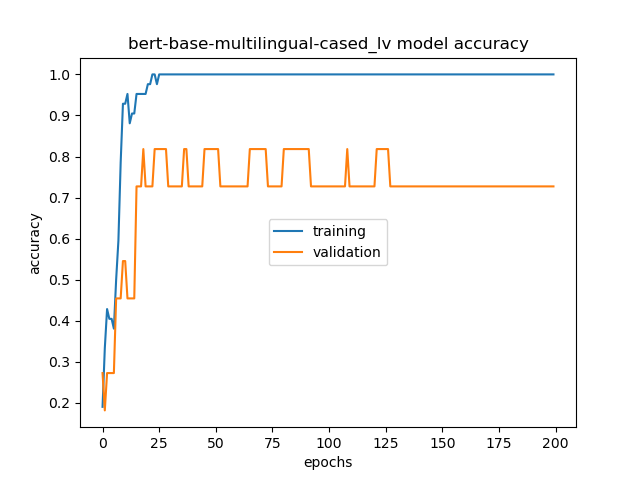
\includegraphics[width=0.49\linewidth,trim={0 0.1cm 0 0},clip]{results-5/graphs/askubuntu_bert-base-multilingual-cased_lv-accuracy.png}}
   \subcaptionbox{mBERT mašīntulkoto latviešu treniņdatu kopa}{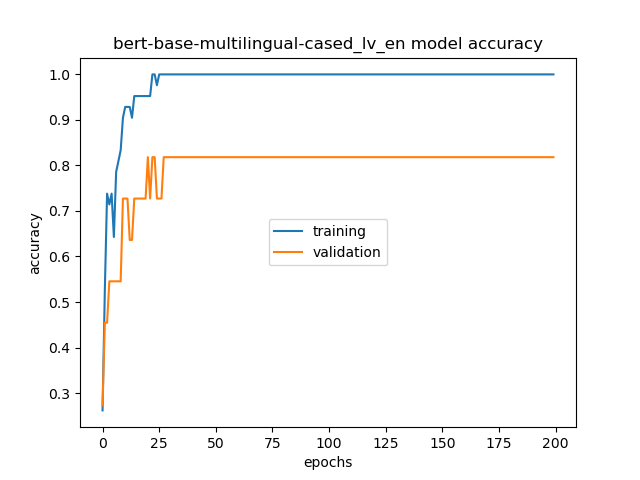
\includegraphics[width=0.49\linewidth,trim={0 0.1cm 0 0},clip]{results-5/graphs/askubuntu_bert-base-multilingual-cased_lv_en-accuracy.png}}
   \caption{caption} 
   \label{fig:askubuntu-bert}
\end{figure}


\begin{figure}[h] 
   \centering
   \subcaptionbox{mBERT apvienotā treniņdatu kopa}{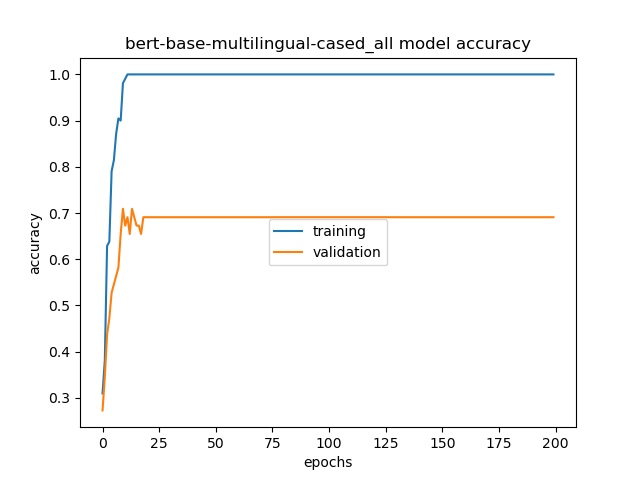
\includegraphics[width=0.49\linewidth,trim={0 0.1cm 0 0},clip]{results-5/graphs/askubuntu_bert-base-multilingual-cased_all-accuracy.png}}
   \subcaptionbox{mBERT apvienotā mašīntulkoto treniņdatu kopa}{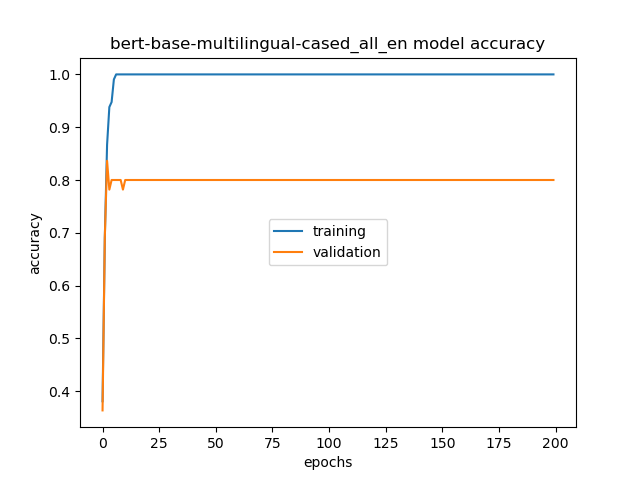
\includegraphics[width=0.49\linewidth,trim={0 0.1cm 0 0},clip]{results-5/graphs/askubuntu_bert-base-multilingual-cased_all_en-accuracy.png}}
   \caption{caption} 
   \label{fig:askubuntu-bert-all}
\end{figure}


\begin{figure}[h] 
   \centering
   \subcaptionbox{mBERT angļu treniņdatu kopa}{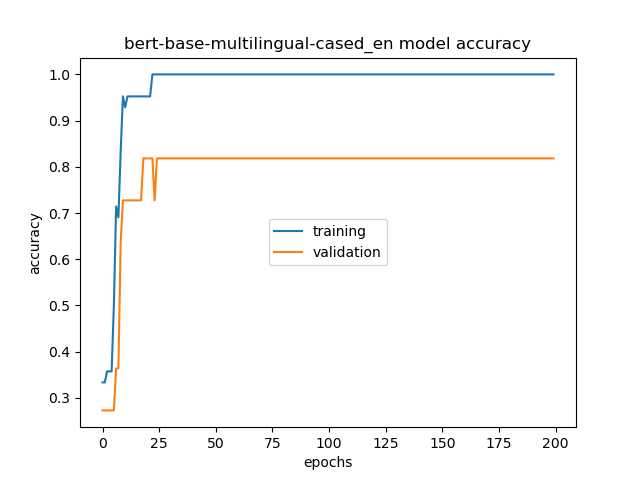
\includegraphics[width=0.49\linewidth,trim={0 0.1cm 0 0},clip]{results-5/graphs/askubuntu_bert-base-multilingual-cased_en-accuracy.png}}
   \subcaptionbox{XLM-RoBERTa angļu treniņdatu kopa}{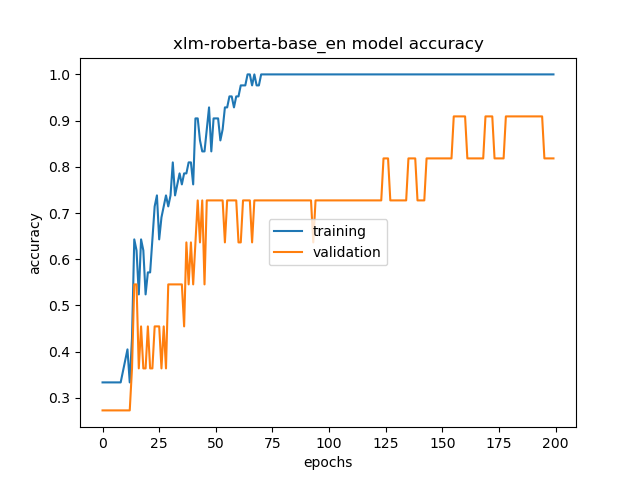
\includegraphics[width=0.49\linewidth,trim={0 0.1cm 0 0},clip]{results-5/graphs/askubuntu_xlm-roberta-base_en-accuracy.png}}
   \caption{caption} 
   \label{fig:askubuntu-bert-xlm-en}
\end{figure}


\begin{figure}[h] 
   \centering
   \subcaptionbox{XLM-RoBERTa latviešu treniņdatu kopa}{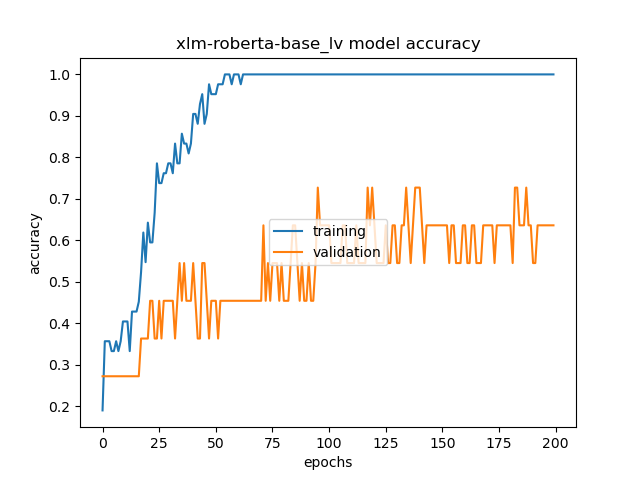
\includegraphics[width=0.49\linewidth,trim={0 0.1cm 0 0},clip]{results-5/graphs/askubuntu_xlm-roberta-base_lv-accuracy.png}}
   \subcaptionbox{XLM-RoBERTa mašīntulkoto latviešu treniņdatu kopa}{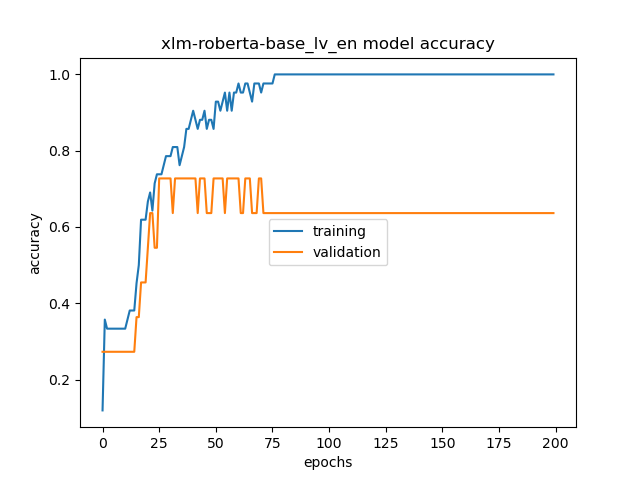
\includegraphics[width=0.49\linewidth,trim={0 0.1cm 0 0},clip]{results-5/graphs/askubuntu_xlm-roberta-base_lv_en-accuracy.png}}
   \caption{caption} 
   \label{fig:askubuntu-xlm}
\end{figure}


\begin{figure}[h] 
   \centering
   \subcaptionbox{XLM-RoBERTa apvienotā treniņdatu kopa}{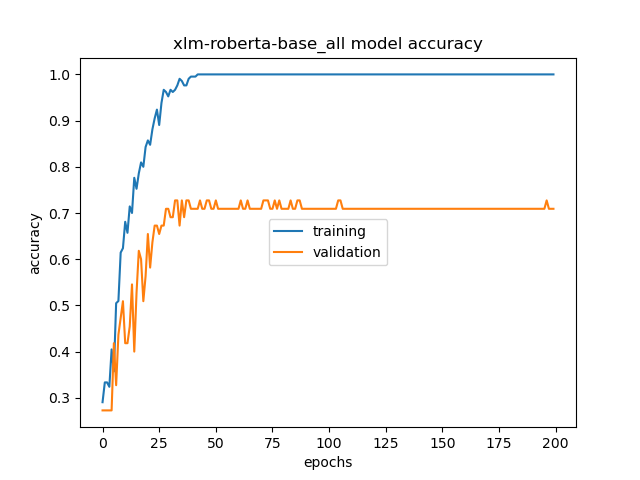
\includegraphics[width=0.49\linewidth,trim={0 0.1cm 0 0},clip]{results-5/graphs/askubuntu_xlm-roberta-base_all-accuracy.png}}
   \subcaptionbox{XLM-RoBERTa apvienotā mašīntulkoto treniņdatu kopa}{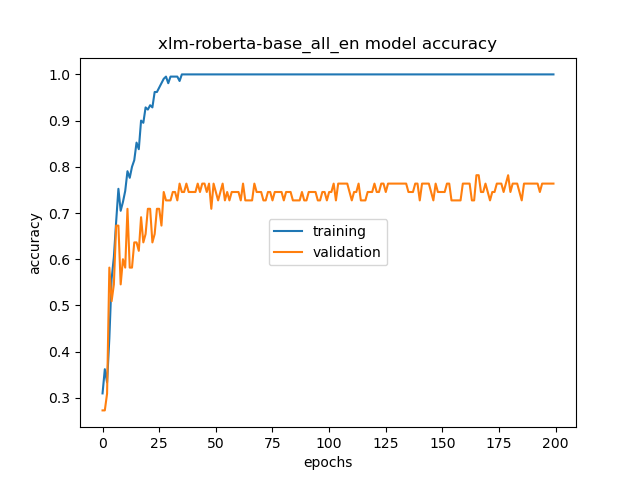
\includegraphics[width=0.49\linewidth,trim={0 0.1cm 0 0},clip]{results-5/graphs/askubuntu_xlm-roberta-base_all_en-accuracy.png}}
   \caption{caption} 
   \label{fig:askubuntu-xlm-all}
\end{figure}



\section{Webapps datu kopa}


Webapps datu kopā ir nodoms ar tikai vienu piemēru, kas izraisa "ValueError: The least populated class in y has only 1 member, which is too few. The minimum number of groups for any class cannot be less than 2." Tāpēc nodomi ar mazāk nekā trīs piemēriem tika apvienoti vienā nodomā "Other". Tas atbilst reālam pielietojumam industrijā, kur nodomi nav vienlīdzīgi pārstāvēti  -- piemēram, starp 115 dažādiem nodomiem divi visbiežākie nodomi kopā pārstāv 33\% datu kopas \cite{paikens2020} -- un ir svarīgi spēt atsijāt nodomus, kurus jāapstrādā klientu apkalpošanas speciālistam -- cilvēkam.




 % The first table shows the accuracy results for mBERT, while the second table shows the results for XLM-RoBERTa. Comparing the two tables, we can see that XLM-RoBERTa performs better than mBERT in most cases. For example, for language 1b (English), XLM-RoBERTa achieves 42.37\% accuracy, while mBERT achieves 64.41\% accuracy. Similarly, for language 3b (Latvian), XLM-RoBERTa achieves 32.20\% accuracy, while mBERT achieves only 61.02% accuracy.

 % Comparing the accuracy results between the two sub-tasks of each language, we can see that in most cases, sub-task 2 performs better than sub-task 1. For example, in language 1a (English), the accuracy for sub-task 1a is not available, while the accuracy for sub-task 2a is 67.80\%. Similarly, in language 3a (Latvian), the accuracy for sub-task 3a is not available, while the accuracy for sub-task 3b is 30.51\%. However, there are some exceptions, such as in language 1b (English), where sub-task 1b has a lower accuracy than sub-task 2b.

 % When comparing the accuracy results across all languages, we can see that Latvian and Russian generally have higher accuracies than the other languages, while Estonian has the lowest accuracy. Additionally, sub-task 2 generally has higher accuracies than sub-task 1.

 % Looking at the individual languages, we can see that the performance varies greatly between the languages. For example, in language 1b (English), mBERT achieves an accuracy of 64.41\%, while XLM-RoBERTa achieves only 42.37\%. However, in language 3b (Latvian), XLM-RoBERTa achieves an accuracy of 32.20\%, while mBERT achieves only 61.02\%. Therefore, the performance of the models depends heavily on the specific language being analyzed.


Salīdzinot abas tabulas, redzams, ka XLM-RoBERTa vairumā gadījumu ir zemāka preciztāte nekā nekā mBERT, bet visaugstākajos rezultātos -- 2a un 2b metodēs XLM-RoBERTa ir pārāks. Šajā gadījumā spēja vienā metodē sasniegt konsekventi labus rezultātus ir svarīgāka nekā viduvēji rezultāti visās, jo pastāv iespēja izvēlēties un lietot vislabāko.

Angļu valodā 1b XLM-RoBERTa ir ar precizitāti 42.37\%, kas varētu būt nejaušība, jo 3b arī apmāca un trenē uz tieši tāda paša korpusa un ir 64.41\%, tāpēc to var neņemt vērā. Ar mBERT jēdzientelpu šāda problēma angļu valodai nebija novērota (apmācot modeli ar 1b metodi tika iegūta precizitāte 64.41\%).

Atšķirībā no pārējām datu kopām nodomu noteikšanas precizitāte igauņu valodā nav sliktāka, salīdzinot ar citām maz-resursu valodām -- igauņu valodai maksimālā precizitāte sasniedz gandrīz 75\%, bet latviešu un lietuviešu valodām tā ir attiecīgi 73\% un 80\%. Tādā veidā maz-resursu valodas uz šīs datu kopas ir ar līdzīgu precizitāti kā krievu valodai, kura ir daudz plašāk pārstāvēta tekstu korpusos.






\begin{table}[htbp]
  \centering
  \caption{Unikālo nodomu skaits ``webapps" treniņkopā un testa kopā. Ar treknrakstu iezīmētas nodomi, kuri ir pietiekami pārstāvētas, pārējie nodomi tika apvienoti vienā jaunā nodomā: "Other"}
    \begin{tabular}{lrrr} \toprule
    Nodoms & Treniņkopā & Testa kopā & $\Sigma$ \\\midrule
    \textbf{Find Alternative} & \textbf{7} & \textbf{16} & 23\\
    \textbf{Delete Account} & \textbf{7} & \textbf{10} & 17\\
    \textbf{Filter Spam} & \textbf{6} & \textbf{14} & 20 \\
    \textbf{Sync Accounts} & \textbf{3} & \textbf{6} & 9 \\
    Change Password & 2     & 6 & 8\\
    None  & 2     & 4 & 6\\
    Export Data & 2     & 3 & 5 \\
    Download Video & 1     & 0 & 1\\
    $\Sigma$ & 30    & 59 & 89 \\\bottomrule
    \end{tabular}%
  \label{tab:webapps-labels}%
\end{table}%


% Table generated by Excel2LaTeX from sheet 'webapps_bert-base-multilingual-'
% \begin{table}[htbp]
%   \centering
%   \caption{Nodomu noteikšanas precizitāte uz \textit{Webapps} datukopas ar mBERT modeli, \%}
%   % \caption{Webapps rezultāti ar mBERT modeli}
%     \begin{tabular}{lrrrrrr}\toprule
%     languages & 1a & 1b & 2a & 2b & 3a & 3b \\\midrule
%     en    &   --  & 64.41 &   --  & 67.80 &  --   & 61.02 \\
%     lv    & 67.80 & 57.63 & 64.41 & 66.10 & 69.49 & 30.51 \\
%     ru    & 67.80 & 69.49 & 72.88 & 74.58 & 64.41 & 44.07 \\
%     et    & 55.93 & 61.02 & 67.80 & 71.19 & 69.49 & 42.37 \\
%     lt    & 62.71 & 49.15 & 67.80 & 66.10 & 66.10 & 28.81 \\\bottomrule
%     \end{tabular}%
%   \label{tab:webapps-bert}%
% \end{table}%


% Table generated by Excel2LaTeX from sheet 'webapps_bert-base-multilingual-'
\begin{table}[htbp]
  \centering
  \caption{Nodomu noteikšanas precizitāte uz \textit{Webapps} datukopas ar mBERT modeli, \%}
    \begin{tabular}{lrrrrrr}\toprule
    languages & 1a & 1b & 2a & 2b & 3a & 3b \\\midrule

    en    &   --  & \cellcolor[rgb]{ .984,  .961,  .973}64.41 &  --   & \cellcolor[rgb]{ .863,  .902,  .957}67.80 &   --  & \cellcolor[rgb]{ .984,  .906,  .918}61.02 \\
    lv    & \cellcolor[rgb]{ .863,  .902,  .957}67.80 & \cellcolor[rgb]{ .984,  .855,  .867}57.63 & \cellcolor[rgb]{ .984,  .961,  .973}64.41 & \cellcolor[rgb]{ .988,  .988,  1}66.10 & \cellcolor[rgb]{ .737,  .812,  .914}69.49 & \cellcolor[rgb]{ .973,  .435,  .443}30.51 \\
    ru    & \cellcolor[rgb]{ .863,  .902,  .957}67.80 & \cellcolor[rgb]{ .737,  .812,  .914}69.49 & \cellcolor[rgb]{ .482,  .631,  .824}72.88 & \cellcolor[rgb]{ .353,  .541,  .776}74.58 & \cellcolor[rgb]{ .984,  .961,  .973}64.41 & \cellcolor[rgb]{ .976,  .647,  .655}44.07 \\
    et    & \cellcolor[rgb]{ .98,  .827,  .839}55.93 & \cellcolor[rgb]{ .984,  .906,  .918}61.02 & \cellcolor[rgb]{ .863,  .902,  .957}67.80 & \cellcolor[rgb]{ .608,  .722,  .867}71.19 & \cellcolor[rgb]{ .737,  .812,  .914}69.49 & \cellcolor[rgb]{ .976,  .62,  .627}42.37 \\
    lt    & \cellcolor[rgb]{ .984,  .933,  .945}62.71 & \cellcolor[rgb]{ .98,  .725,  .733}49.15 & \cellcolor[rgb]{ .863,  .902,  .957}67.80 & \cellcolor[rgb]{ .988,  .988,  1}66.10 & \cellcolor[rgb]{ .988,  .988,  1}66.10 & \cellcolor[rgb]{ .973,  .412,  .42}28.81 \\\bottomrule
    avg   & 63.56 & 60.34 & 68.22 & 69.15 & 67.37 & 41.36 \\
    % avg ru-en & 67.80 & 66.95 & 72.88 & 71.19 & 64.41 & 52.54 \\
    avg lv-lt-et & 62.15 & 55.93 & 66.67 & 67.80 & 68.36 & 33.90 \\
    \end{tabular}%
  \label{tab:webapps-bert}%
\end{table}%

% Table generated by Excel2LaTeX from sheet 'webapps_xlm-roberta-base_result'
% \begin{table}[htbp]
%   \centering
%   \caption{Nodomu noteikšanas precizitāte uz \textit{Webapps} datukopas ar XLM-RoBERTa modeli, \%}
%     \begin{tabular}{lrrrrrr}\toprule
%     languages & 1a & 1b & 2a & 2b & 3a & 3b \\\midrule

%     en    &  --   & 42.37 &   --  & 69.49 &   --  & 64.41 \\
%     lv    & 37.29 & 50.85 & 69.49 & 72.88 & 45.76 & 32.20 \\
%     ru    & 35.59 & 44.07 & 71.19 & 67.80 & 42.37 & 38.98 \\
%     et    & 32.20 & 44.07 & 74.58 & 62.71 & 50.85 & 37.29 \\
%     lt    & 62.71 & 50.85 & 79.66 & 67.80 & 59.32 & 32.20 \\\bottomrule
%     \end{tabular}%
%   \label{tab:webapps-xml}%
% \end{table}%


% Table generated by Excel2LaTeX from sheet 'webapps_xlm-roberta-base_result'
\begin{table}[htbp]
  \centering
  \caption{Nodomu noteikšanas precizitāte uz \textit{Webapps} datukopas ar XLM-RoBERTa modeli, \%}
    \begin{tabular}{lrrrrrr}\toprule
    languages & 1a & 1b & 2a & 2b & 3a & 3b \\\midrule

    en    &   --    & \cellcolor[rgb]{ .98,  .725,  .733}42.37 &  --     & \cellcolor[rgb]{ .58,  .702,  .859}69.49 &  --     & \cellcolor[rgb]{ .69,  .78,  .898}64.41 \\
    lv    & \cellcolor[rgb]{ .976,  .569,  .576}37.29 & \cellcolor[rgb]{ .988,  .988,  1}50.85 & \cellcolor[rgb]{ .58,  .702,  .859}69.49 & \cellcolor[rgb]{ .506,  .647,  .831}72.88 & \cellcolor[rgb]{ .98,  .827,  .839}45.76 & \cellcolor[rgb]{ .973,  .412,  .42}32.20 \\
    ru    & \cellcolor[rgb]{ .973,  .514,  .522}35.59 & \cellcolor[rgb]{ .98,  .776,  .788}44.07 & \cellcolor[rgb]{ .541,  .675,  .843}71.19 & \cellcolor[rgb]{ .616,  .725,  .871}67.80 & \cellcolor[rgb]{ .98,  .725,  .733}42.37 & \cellcolor[rgb]{ .976,  .62,  .627}38.98 \\
    et    & \cellcolor[rgb]{ .973,  .412,  .42}32.20 & \cellcolor[rgb]{ .98,  .776,  .788}44.07 & \cellcolor[rgb]{ .467,  .624,  .82}74.58 & \cellcolor[rgb]{ .729,  .808,  .91}62.71 & \cellcolor[rgb]{ .988,  .988,  1}50.85 & \cellcolor[rgb]{ .976,  .569,  .576}37.29 \\
    lt    & \cellcolor[rgb]{ .729,  .808,  .91}62.71 & \cellcolor[rgb]{ .988,  .988,  1}50.85 & \cellcolor[rgb]{ .353,  .541,  .776}79.66 & \cellcolor[rgb]{ .616,  .725,  .871}67.80 & \cellcolor[rgb]{ .804,  .859,  .937}59.32 & \cellcolor[rgb]{ .973,  .412,  .42}32.20 \\\bottomrule
    avg   & 41.95 & 46.44 & 73.73 & 68.14 & 49.58 & 41.02 \\
    % avg en-ru & 35.59 & 43.22 & 71.19 & 68.64 & 42.37 & 51.69 \\
    avg lv-lt-et & 44.07 & 48.59 & 74.58 & 67.80 & 51.98 & 33.90 \\
    \end{tabular}%
  \label{tab:webapps-xml}%
\end{table}%



\begin{figure}[h] 
   \centering
   \subcaptionbox{mBERT latviešu treniņdatu kopa}{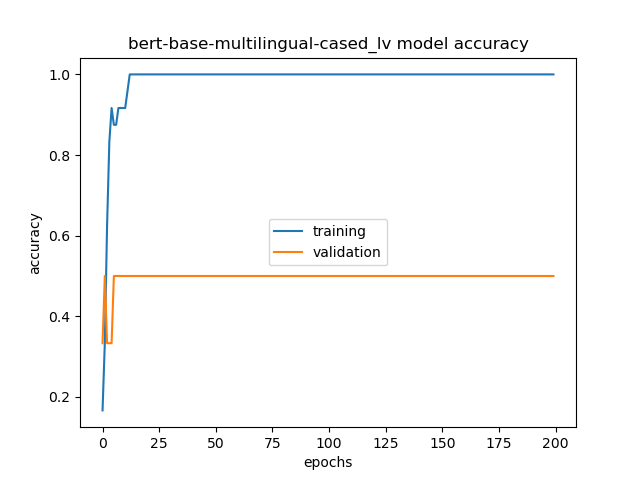
\includegraphics[width=0.49\linewidth,trim={0 0.1cm 0 0},clip]{results-5/graphs/webapps_bert-base-multilingual-cased_lv-accuracy.png}}
   \subcaptionbox{mBERT mašīntulkoto latviešu treniņdatu kopa}{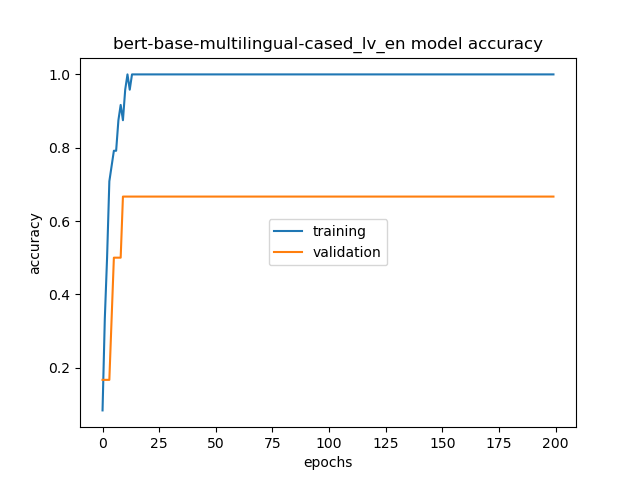
\includegraphics[width=0.49\linewidth,trim={0 0.1cm 0 0},clip]{results-5/graphs/webapps_bert-base-multilingual-cased_lv_en-accuracy.png}}
   \caption{caption} 
   \label{fig:webapps-bert}
\end{figure}


\begin{figure}[h] 
   \centering
   \subcaptionbox{mBERT apvienotā treniņdatu kopa}{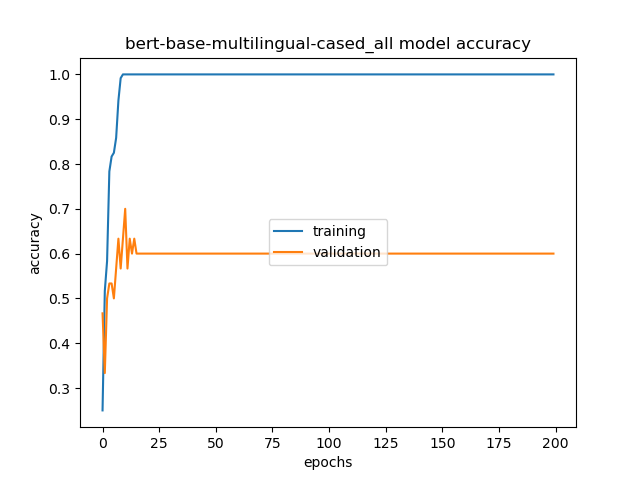
\includegraphics[width=0.49\linewidth,trim={0 0.1cm 0 0},clip]{results-5/graphs/webapps_bert-base-multilingual-cased_all-accuracy.png}}
   \subcaptionbox{mBERT apvienotā mašīntulkoto treniņdatu kopa}{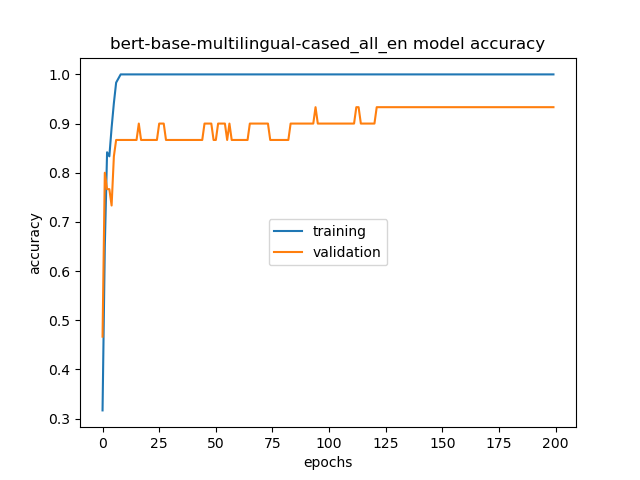
\includegraphics[width=0.49\linewidth,trim={0 0.1cm 0 0},clip]{results-5/graphs/webapps_bert-base-multilingual-cased_all_en-accuracy.png}}
   \caption{caption} 
   \label{fig:webapps-bert-all}
\end{figure}


\begin{figure}[h] 
   \centering
   \subcaptionbox{mBERT angļu treniņdatu kopa}{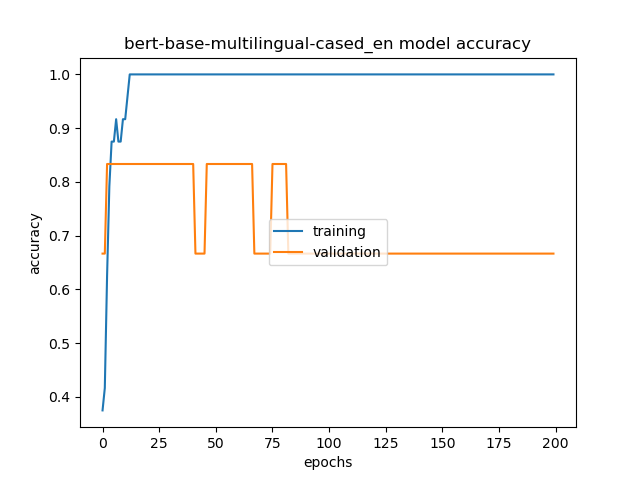
\includegraphics[width=0.49\linewidth,trim={0 0.1cm 0 0},clip]{results-5/graphs/webapps_bert-base-multilingual-cased_en-accuracy.png}}
   \subcaptionbox{XLM-RoBERTa angļu treniņdatu kopa}{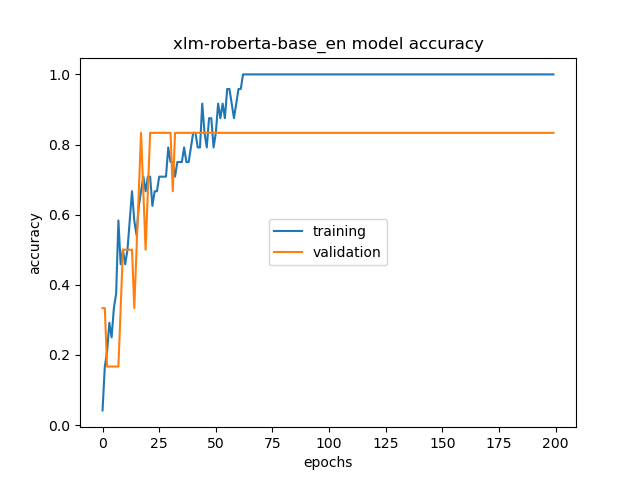
\includegraphics[width=0.49\linewidth,trim={0 0.1cm 0 0},clip]{results-5/graphs/webapps_xlm-roberta-base_en-accuracy.png}}
   \caption{caption} 
   \label{fig:webapps-bert-xlm-en}
\end{figure}


\begin{figure}[h] 
   \centering
   \subcaptionbox{XLM-RoBERTa latviešu treniņdatu kopa}{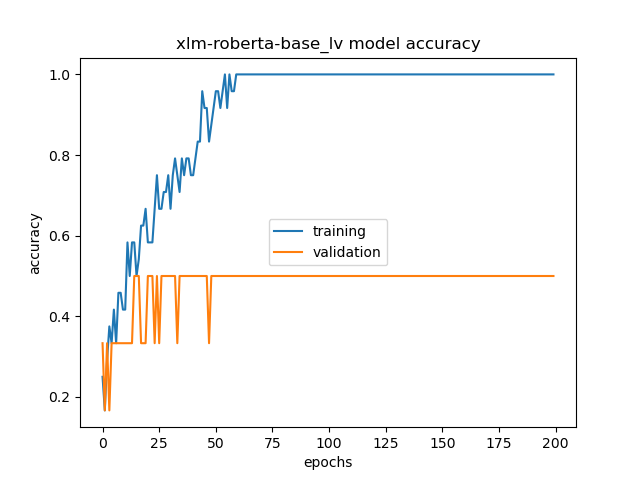
\includegraphics[width=0.49\linewidth,trim={0 0.1cm 0 0},clip]{results-5/graphs/webapps_xlm-roberta-base_lv-accuracy.png}}
   \subcaptionbox{XLM-RoBERTa mašīntulkoto latviešu treniņdatu kopa}{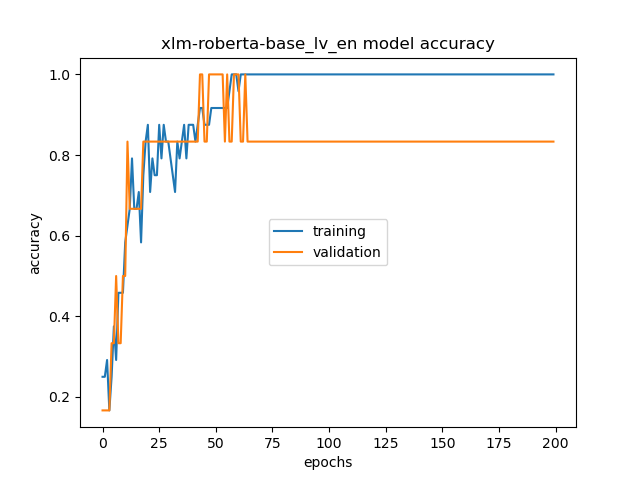
\includegraphics[width=0.49\linewidth,trim={0 0.1cm 0 0},clip]{results-5/graphs/webapps_xlm-roberta-base_lv_en-accuracy.png}}
   \caption{caption} 
   \label{fig:webapps-xlm}
\end{figure}


\begin{figure}[h] 
   \centering
   \subcaptionbox{XLM-RoBERTa apvienotā treniņdatu kopa}{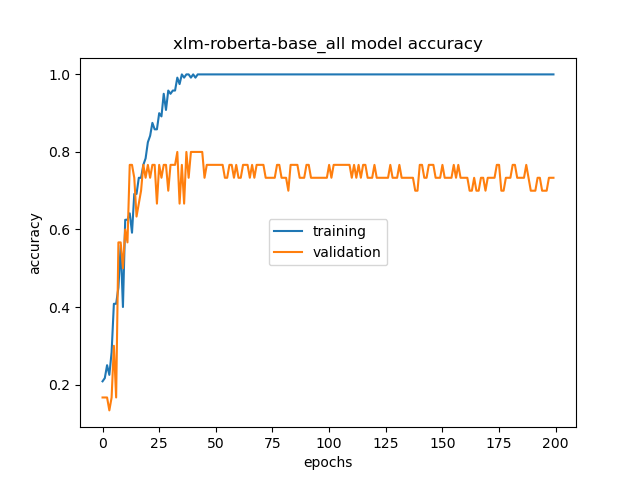
\includegraphics[width=0.49\linewidth,trim={0 0.1cm 0 0},clip]{results-5/graphs/webapps_xlm-roberta-base_all-accuracy.png}}
   \subcaptionbox{XLM-RoBERTa apvienotā mašīntulkoto treniņdatu kopa}{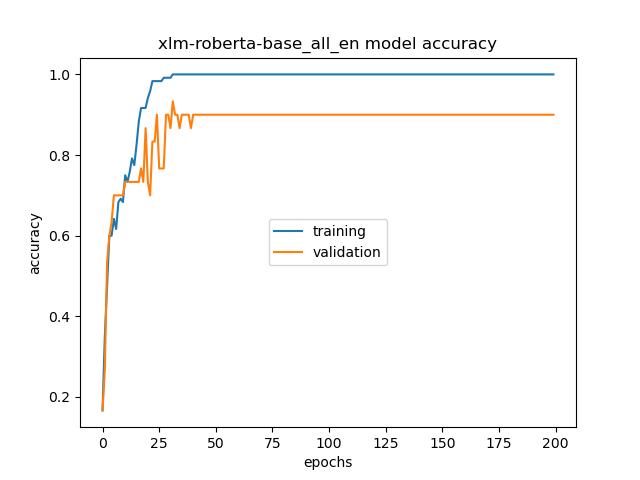
\includegraphics[width=0.49\linewidth,trim={0 0.1cm 0 0},clip]{results-5/graphs/webapps_xlm-roberta-base_all_en-accuracy.png}}
   \caption{caption} 
   \label{fig:webapps-xlm-all}
\end{figure}




% \chapter*{Secinājumi}
% \addcontentsline{toc}{chapter}{Secinājumi}
% % \begin{itemize}
%     \item \textit{Chatbot};
%     \item \textit{Askubuntu};
%     \item \textit{Webapps}.
% \end{itemize}


% \begin{itemize}
%     \item mBERT;
%     \item XLM-RoBERTa.
% \end{itemize}

% \begin{itemize}
%     \item oriģinālvalodā;
%     \item mašīntulkojumā uz angļu valodu.
% \end{itemize}


% \begin{itemize}
%     \item uz tās pašas valodas korpusa;
%     \item uz visu piecu valodu korpusa;
%     \item tikai uz angļu valodas korpusa.
% \end{itemize}


Vislabākie nodomu noteikšanas precizitātes rezultāti ir \textit{Chatbot} datu kopā, tālāk iet \textit{Askubuntu} un \textit{Webapps}. Tādā pašā secībā iet šīs datu kopas pēc korpusa apjoma (206, 162 un 89 lietotāju ievadi attiecīgi), un līdzīgi sadalās piemēru skaits vienam nodomam. \textit{Chatbot} datu kopā visu metožu (izņemot 3b) vidējie rezultāti ir būtiski pārāki par \textit{Askubuntu} un \textit{Webapps} rezultātiem. Vairāk datu ir lielāka ietekme (\textit{impact}) uz precizitāti nekā vislabākās metodes izvēle.

mBERT jēdzientelpām ir labāka precizitāte \textit{Askubuntu} un \textit{Webapps} datu kopās, bet XLM-RoBERTa ir labāka precizitāte \textit{Chatbot} datu kopā.

Mašīntulkošana uz angļu valodu ir izdevīga stratēģija (četri a labākie vidējie rezultāti pret diviem b, skat. \ref{tab:avg-method}. tabula). Lai arī nodomu noteikšanas korpusā visas valodas ir vienādi pārstāvētas, daudzvalodu jēdzientelpu modeļi ir apmācīti uz procentuāli lielākas daļas angļu valodas teksta. Mašīntulkošanas pārākums par oriģinālvalodu šajā kontekstā ir interesants, jo mašīntulkošana rada papildu trokšņus un kļūdas un ``pazaudē tulkojumā" katrai valodai svarīgās nianses, kas var ietekmēt ievades datu kvalitāti.

Skaitliski mazākās datu kopās (\textit{Askubuntu} un \textit{Webapps}) apvienot treniņdatus vienā ir laba ideja, trijos no četriem gadījumiem labākais vidējais rezultāts bija metodē, kurā ne-angļu treniņdati tika mašīntulkoti uz angļu valodu. Stabili vissliktākā metode ir apmācīt datus tikai uz angļu valodas korpusa un testēt uz korpusa citā valodā, pirms tam netulkojot uz angļu valodu. Iespējams tas ir saistīts ar šo korpusu specifiku (maz datu). Taču 3b ir interesanta metode, jo parāda starpvalodu mācīšanos. 

Līdzīgu datu korpusu gadījumā virtuālajam asistentam autors izvēlētos trenēt vienu nodomu klasifikācijas modeli, kas apmācīts uz datiem, kas ir mašīntulkoti uz angļu valodu un apvienoti vienā korpusā.



% Datu kopas



% Table generated by Excel2LaTeX from sheet 'Sheet1'
% \begin{table}[htbp]
%   \centering
%   \caption{Add caption}
%     \begin{tabular}{rlrrrrrr}
%           &       & \multicolumn{1}{l}{1a} & \multicolumn{1}{l}{1b} & \multicolumn{1}{l}{2a} & \multicolumn{1}{l}{2b} & \multicolumn{1}{l}{3a} & \multicolumn{1}{l}{3b} \\
%     \multicolumn{1}{l}{chatbot} & mbert & 91.39 & 92.03 & 92.16 & 92.08 & \textbf{92.57} & 81.98 \\
%           & roberta & 90.45 & 91.93 & 92.69 & \textbf{93.54} & 91.16 & 84.62 \\
%     \multicolumn{1}{l}{askubuntu} & mbert & 79.87 & \textbf{81.10} & 79.24 & 79.95 & 79.36 & 62.84 \\
%           & roberta & 66.92 & 68.90 & \textbf{77.12} & 76.74 & 68.75 & 52.94 \\
%     \multicolumn{1}{l}{webapps} & mbert & 64.72 & 63.14 & \textbf{73.20} & 67.29 & 62.71 & 42.71 \\
%           & roberta & 43.64 & 49.24 & \textbf{66.31} & 66.10 & 48.62 & 35.85 \\
%     \end{tabular}%
%   \label{tab:addlabel}%
% \end{table}%



\begin{table}[htbp]
  \centering
  \caption{Visu valodu vidējie rezultāti katrai metodei visās jēdzientelpās un datu kopās, \%.}
    \begin{tabular}{rlrrrrrr}\toprule
          &       & 1a    & 1b    & 2a    & 2b    & 3a    & 3b \\\midrule
    \textit{Chatbot} & mBERT & 91.39 & 92.03 & 92.16 & 92.08 & \textbf{92.57} & 81.98 \\
          & XLM-RoBERTa & 90.45 & 91.93 & 92.69 & \textbf{93.54} & 91.16 & 84.62 \\\midrule
    \textit{Askubuntu} & mBERT & 79.87 & \textbf{81.10} & 79.24 & 79.95 & 79.36 & 62.84 \\
          & XLM-RoBERTa & 66.92 & 68.90 & \textbf{77.12} & 76.74 & 68.75 & 52.94 \\\midrule
    \textit{Webapps} & mBERT & 64.72 & 63.14 & \textbf{73.20} & 67.29 & 62.71 & 42.71 \\
          & XLM-RoBERTa & 43.64 & 49.24 & \textbf{66.31} & 66.10 & 48.62 & 35.85 \\\bottomrule
    \end{tabular}%
  \label{tab:avg-method}%
\end{table}%



% \chapter*{Pateicības}
% \addcontentsline{toc}{chapter}{Pateicības}
% Paldies Aleksandrai Elbakjanai par sci-hub.



\clearpage
\addcontentsline{toc}{chapter}{Izmantotā literatūra un avoti}
\printbibliography[title=Izmantotā literatūra un avoti]

\clearpage

\appendix
\chapter*{Pielikums}
\addcontentsline{toc}{chapter}{Pielikums}
% the \\ insures the section title is centered below the phrase: AppendixA
%\noindent {\large \textbf{Dalība konferencēs}}

\noindent {\large \textbf{Kods}}\\
Koda piemērs literatūras ievadā.
Krāsu dati "xkcd.json"
\url{https://github.com/dariusk/corpora/blob/master/data/colors/xkcd.json}.\\
Ideja un hex\_to\_int un closest funkcijas \cite{parrish2017}, pārējās pārrakstītas ātrdarbībai ar numpy.

\begin{python}[basicstyle=\tiny]
import numpy as np
import json

def hex_to_int(s):
    s = s.lstrip("#")
    return int(s[:2], 16), int(s[2:4], 16), int(s[4:6], 16)


def distance(coord1, coord2):
	"""Euclidean distance between two points
	"""
	return np.sqrt(np.sum(np.subtract(coord1, coord2)**2))


def subtractv(coord1, coord2):
	"""coord1 - coord2
	"""
	return np.subtract(coord1, coord2)


def addv(coord1, coord2):
	"""coord1 + coord2
	"""
	return np.sum([coord1, coord2], axis=0)


def closest(space, coord, n=10):
	closest = []
	for key in sorted(space.keys(),
					  key=lambda x: distance(coord, space[x]))[:n]:
		closest.append(key)
	return closest


color_data = json.loads(open("xkcd.json").read())

colors = dict()
for item in color_data['colors']:
    colors[item["color"]] = hex_to_int(item["hex"])
\end{python}

% Dokumentālā lapa
% \makedoklapa

\end{document}
